\chapter{Homology}
\label{chapter5}

In this chapter we will shift our attention back to algebraic topology and cover the last pieces of background material we need. Those are Homology and Persistent Homology. We will introduce Homology and as tool to analyse the connectivity and number of the holes and voids in a simplical complex. Using Homology we will define the concept of Persistent Homology. Persistent homology makes use of homology to analyse how the connectivity of a simplicial complex changes as we attach new cells to it.

\section{Homology}

The guiding principle behind the Euler Characteristic was to decompose a space into cells, count them and perform cancellations based on the parity of the dimension of the cells. This approach yields valuable information about a topological space, but we can hope to gain more by generalising it. We shall accomplish this by leveraging the mathematical machinery of Homology. Homology is a tool that was first developed to measure the topological complexity of manifolds \cite{persistence-original}. For example with homology we can recognize that there is a hole in the torus and a 3-dimensional volume enclosed in the sphere. The theory of Homology comes in two flavours - \textbf{simplical} and \textbf{singular}. Simplicial homology is geared towards analysing simplical complexes and singular homology its generalisation to arbitrary topological spaces. In this dissertation we will restrict our attention to singular homology because we are primarily interested in the computational aspect of homology.

%We will however on occasion refer to singular homology when we desire to leverage a more general result from the relevant theory. More information on singular homology can be found in the following sources \cite{algebraic-topology, elementary-applied-topology}
\begin{figure}[h]%
    \centering
    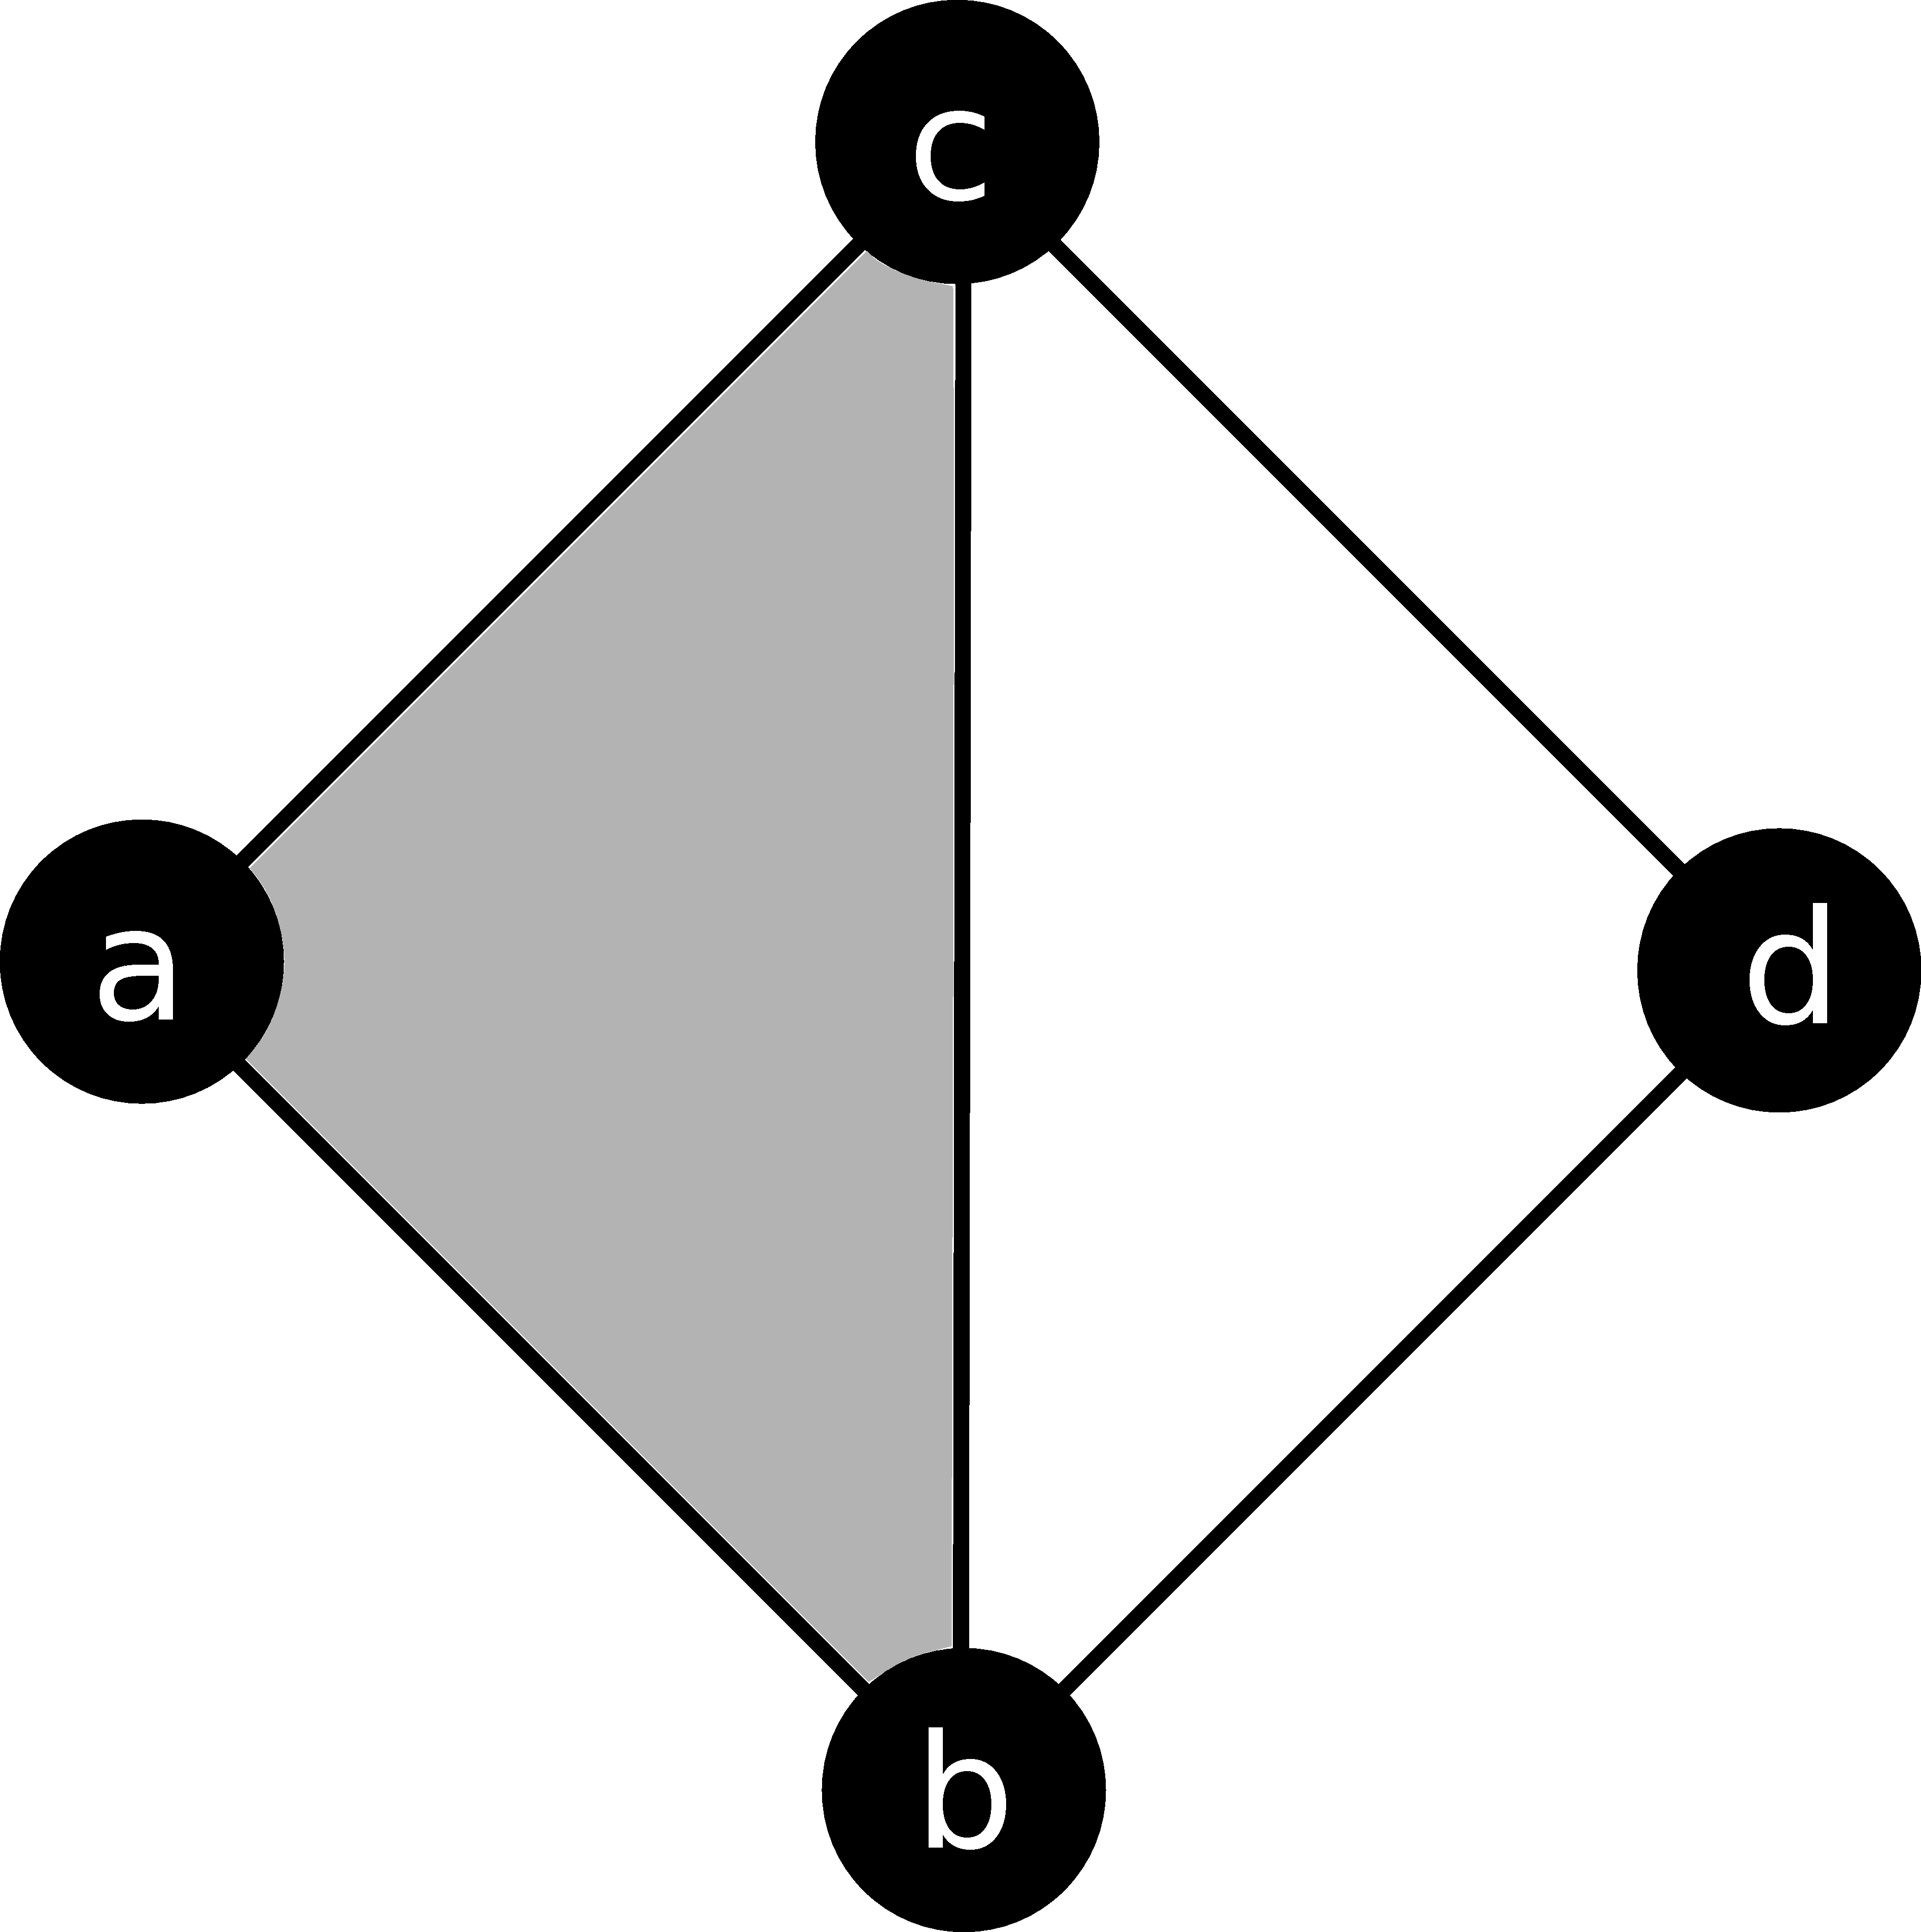
\includegraphics[scale=0.08]{./images/simplex/complex-romb.pdf}%
    \caption{A simplical complex.}%
    \label{fig:hom-sc}%
\end{figure}

Homology is built around the interplay between the two key concepts of \textbf{cycles} and \textbf{boundaries}. Let us consider the simplical complex depicted on Figure \ref{fig:hom-sc} as an example. It consists of four vertices $\{a, b, c, d\}$, five edges $\{ab, bc, ac, bd, bc\}$ and one face $\{abc\}$. Let us first explain what a boundary is. The boundary of a simplex consists of all faces of the simplex whose dimension is one less. We will also call these the codimension-1 faces of the simplex. For example the boundary of the 1-dimensional simplex (1-simplex) $ab$ consists of the 0-simplices $a \text{ and } b$. The boundary of the 2-simplex $abc$ consists of the 1-simplices $ab, ac \text{ and } bc$.

A cycle consists of the simplices that form the boundary of a simplex that is of one dimension higher (regardless of whether that simplex is in the complex). In our example we can observe that the edges $ab, bc, ac$ and $bd, cd, bc$ form a 1-dim cycle (1-cycle) because they are the boundary of the 2-simplices $abc$ and $bcd$. The first simplex $abc$ is in the complex while $bcd$ is not. The definition of one dimensional cycles is similar to the graph theoretic definition of a cycle. The first and last vertex of the paths formed by those edges are the same. A more geometric way explain this is to say that a 1-cycles is a set of edges that completely enclose a 2-dimensional area. To expand this definition to higher dimensional cycles consider the codimension-1 faces of a tetrahedron (four triangles). They form a 2-cycle as they completely enclose a 3-dimensional volume. In general an n-cycle consists of simplices that are the boundary of a (n+1)-simplex.

The interplay between between cycles and boundaries is best described by the following question. Which cycles in the complex are \textbf{not} the boundary of a higher dimensional simplex? Such cycles are important because they introduce a void in the complex. Cycles which are the boundary of a higher dimensional simplex can be disregarded because the void they introduce is filled by that higher dimensional simplex. Coming back to our example the cycle $ab, bc, ac$ is the boundary of the 2-simplex $abc$, but the cycle $bd, cd, bc$ it not the boundary of a simplex that is in the simplical complex. The cycle $bd, cd, bc$ represents a 2-dimensional hole in the simplical complex. Note that the cycle $ab, bd, cd, ac$ is in a sense equivalent to the cycle $bd, cd, bc$ because both describe the same 2-dimensional hole in the complex - namely the missing 2-simplex $bcd$.

Finally observe that the paths formed by the edges $bc, ac, ab$ and $ac, ab, bc$ represent the same cycle. The only difference is which vertex is the starting and ending point. To emphasise that these two cycles are the same we will completely disregard the concept of starting and ending point in a cycle by introducing additive algebraic notation. In this notation the same cycle would be written as $ab + bc + ca$.

Additive notation implies associativity but it does not have the sole purpose of illustrating the point of disregarding edge order. Its more important aspect is that it allows us to treat sums of edges as linear combinations in an abstract vector space. We will work with vector spaces over the field of coefficients $\mathbb{Z}_2 = \{0, 1\}$ together with the standard operations of addition and multiplication modulo two. We will call the elements of these vector spaces n-chains.

Let $X$ be a simplicial complex. An n-chain of $X$ is a formal sum of n-simplices of $X$ \cite{comp-topo}. The notation we will use for an n-chain is $\sum{a_i \sigma_i}$ where $a_i \in \mathbb{Z}_2$ and $\sigma_i$ is an n-simplex of $X$. We can add two n-chains component wise much like we would add polynomials. For example $(ab + bc) + (ab + cd + bd) = 2ab + bc + cd + bd = bc + cd + bd$ because $2 = 0$ in $\mathbb{Z}_2$. Based on the n-chains of $X$ we can define the \em chain complex \em of $X$. It is made up of the following vector spaces and linear maps between them:

% We will use abstract vector spaces over the field of coefficients $\mathbb{Z}_2$ as the building blocks of our study of Homology.

\begin{itemize}

    \item The \textbf{group of n-chains} $C_n(X)$ of $X$. These are vector spaces where the vectors are all possible n-chains of $X$ and the coefficients are $\mathbb{Z}_2$.

    \item The \textbf{boundary maps} $\partial_n$ between the groups of n-chains of $X$. These are linear maps between consecutive groups of n-chains $\partial_n : C_n(X) \to C_{n-1}(X)$.

\end{itemize}

What we have defined as the chain complex of $X$ is no more that a collection of vector spaces together with linear maps between. When $n$ is smaller than zero or bigger than the dimension of $X$ then the vector spaces $C_n(X)$ are trivial. They consisting only of the zero element. We can visualise the chain complex of $X$ with the so called quiver representation. For our example simplical complex it would look like:

$$ 0 \overset{\partial_{3}}{\longrightarrow} C_2(X) \overset{\partial_{2}}{\longrightarrow} C_{1}(X) \overset{\partial_{1}}{\longrightarrow} C_{0}(X) \overset{\partial_0}{\longrightarrow}  0 $$

In the general case for an n-dimensional simplical complex $X$ the full chain complex would be:

$$ ... \longrightarrow 0 \overset{\partial_{n+1}}{\longrightarrow} C_n(X) \overset{\partial_{n}}{\longrightarrow} C_{n-1}(X) \overset{\partial_{n-1}}{\longrightarrow} ... \longrightarrow  \overset{\partial_1}{\longrightarrow} C_0(X) \overset{\partial_0}{\longrightarrow} 0 \longrightarrow ... $$
where we can extend both the right and left-hand sides with the zero vector spaces and zero maps infinitely. More specifically in this sequence $\partial_{n+1} \text{ and } \partial_{0}$ are zero maps. The boundary map $\partial_{n+1}$ sends the zero vector of $0$ to the zero vector of $C_n(X)$ and the map $\partial_0$ sends all vectors in $C_0(X)$ to the zero vector in $0$.

Let us now explain how the groups of n-chains and the boundary maps of a simplical complex are constructed explicitly. In our working example $C_0(X)$ is the vector space that is spanned by all possible linear combinations of the vertices $\{a, b, c, d\}$ of the complex. Therefore $\{a, b, c, d\}$ is a basis for $C_0(X)$ and we write this as $C_0(X) = span(\{a, b, c, d\})$. A vector in $C_0(X)$ is a linear combination of the basis vectors using coefficients in $\mathbb{Z}_2$. Let $\sigma \in C_0(X)$ be an 0-chain, then we can express it as $\sigma  = \alpha_0a + \alpha_1b + \alpha_2c + \alpha_3d$ where $\alpha_i \in \{0 ,1\}$ for every $i = 0, 1, 2, 3$.

Going a dimension up $C_1(X) = span(\{ab, bc, ac, cd, bd\})$. As we pointed out earlier the cycle that consists of the edges $bc, cd, bd$ is represented by the sum or linear combination $bc + cd + bd = 0ab + 1bc + 0ca + 1cd + 1bd$ and has coordinates $(0, 1, 0, 1, 1)$ in $C_1(X)$ with respect to the basis $\{ab, bc, ac, cd, bd\}$. We may of course work use a different basis for the groups of n-chains. For example $C_0(X) = span(\{a + b, b, c, c + d\})$ because the vectors $(1, 1, 0, 0), (0, 1, 0, 0), (0, 0, 1, 0) \text { and } (0, 0, 1, 1,)$ are linearly independent. In this basis the 0-simplex $a + b + c + d$ has coordinates $(1, 0, 0 1)$.

The boundary maps are defined analogously to how we presented them in the beginning of the section. The effect a boundary map has on a simplex $\sigma \in C_n(X)$ is that it returns the linear combination of the simplices of $C_{n-1}(X)$ that are codimension-1 faces of $\sigma$. If $\sigma$ is the convex  combination of the vertices $[v_0, v_1, ..., v_n]$ then we define its boundary as

$$ \partial(\sigma) = \partial([v_0, v_1, ..., v_n]) = \sum_{i=0}^{n}[v_0, ... , \hat{v_i}, ..., v_n] ,$$
where the hat on top of $v_i$ in the sum signifies that we omit it in the convex combination. From this definition we can extend $\partial$ to all n-chains in $C_n(X)$ linearly by allowing it commute with vector addition and scalar multiplication like so:

$$ \partial\bigg(\sum_{\sigma}a_{\sigma}\sigma\bigg) = \partial\bigg(\sum_{\sigma}{a_{\sigma}[v_{\sigma_0}, v_{\sigma_1}, ..., v_{\sigma_n}]}\bigg) = \sum_{\sigma}{a_{\sigma} \sum_{i=0}^{n}[v_{\sigma_0},..., \hat{v}_{\sigma_i}, ..., v_{\sigma_n}]} .$$

Going back to our working example on Figure \ref{fig:hom-sc} let $\sigma = ab + bc + ac$ be an n-chain in $C_1(X)$. Then $\partial(ab + bc + ac) = \partial(ab) + \partial(bc) + \partial(ac) = a + b + b + c + a + c = 2a + 2b + 2c = 0$. This examples allows us to observe an important fact. We know that the n-chain $ab + bc + ca$ is a cycle and we obtained that its boundary is zero. This is no coincidence. The defining feature of a cycles is that they have zero boundary. The n-cycles in $C_{n}(X)$ are defined as the n-chains that go to zero under the boundary map. The set of all vectors that go to zero under a linear map is known as the kernel of the linear map. The kernel of the boundary map $\partial_n : C_{n}(X) \to C_{n-1}(X)$ is denoted as:

$$ Z_n = ker(\partial_n) = \Big\{\sigma \in C_{n}(X): \partial_n\big(\sigma\big) = 0 \Big\}. $$

We can also translate the boundaries in the language of linear algebra. The boundaries in $C_n(X)$ are given by the image of $C_{n+1}(X)$ under $\partial_{n+1}$. We write this as:


$$ B_n = im(\partial_{n+1}) = \Big\{\partial_{n+1}(\sigma) \in C_{n}(X): \sigma \in C_{n+1}(X) \Big\}. $$


%Let us now translate the geometric intuition we have of cycles and boundaries to domain of linear algebra. The boundaries are provided to us by the boundary maps. Thus the set of all boundaries in $C_n(X)$ is given by the image of $C_{n+1}(X)$ under $\partial_{n+1}$ or $im(\partial_{n+1})$. The cycles in $C_n(X)$ are given by all the vectors in $C_n(X)$ that go to the zero vector of $C_{n-1}(X)$ under $\partial_n$. Intuitively the boundary of an n-chain is zero exactly when all of the faces of the simplices in the chain have even parity and cancel in our binary algebra. The set of all vectors that go to the zero vector under the boundary map $\partial$ is precisely the kernel of $\partial$ or $ker(\partial)$.

%From linear algebra we know that for a linear function $f: V \to W$, $ker(f)$ is a linear subspace of $V$ and $im(f)$ is a subspace of $W$. In the context of chain complexes this means that the images and kernels of all the boudary maps are linear subspaces of their respective n-chains. Before learning how the interplay between cycles and boundaries is translated in this setting we must present the following fundamental theorem

Now that we have the means of describing the cycles and boundaries the only thing that we are missing is a way to partition the cycles into groups that differ from each other only by their boundary. This would make precise the notion that the cycles $ab, bd, cd, ac$ and $bd, cd, bc$ in Figure \ref{fig:hom-sc} are equivalent because they both represent hole caused by the missing simplex $bcd$. We must first understand how $Z_n$ and $B_n$ are related through the fundamental Lemma of Homology.

\begin{lem} (Fundamental Lemma of Homology) $\partial_{n-1}(\partial_n(\sigma)) = 0, \text{ for every } \sigma \in C_{n}(X)$. \end{lem}

\begin{proof}
    We will only sketch the intuitive outline of the proof and refer the reader to \cite{algebraic-topology} for a more comprehensive version.

    Let us consider the boundary of $\sigma \in C_n(X)$ which is $\partial_n(\sigma)$. It contains all of the n-1 faces of $\sigma$. Furthermore every n-2 face of $\sigma$ belongs to exactly two n-1 faces of $\sigma$. Therefore they will cancel out in the second boundary operation $\partial_{n-1}(\partial_n(\sigma)) = 0$.
\end{proof}


\begin{cor}  For every two consecutive boundary maps $\partial_n$ and $\partial_{n-1}$ in a chain complex $im(\partial_n) \subseteq ker(\partial_{n-1})$. \end{cor}

\begin{proof}
    If the image of $\partial_n$ were not in the kernel of $\partial_{n-1}$ then there would be at least one n-chain $\sigma$ for which $\partial_{n-1}(\partial_n(\sigma)) \ne 0$. By the Fundamental Lemma of Homology this is not possible.
\end{proof}



Since $B_n = im(\partial_{n+1})$ and $Z_n = ker(\partial_n)$ then $B_n$ is a subset of $Z_n$. We can make an even stronger statement. From linear algebra \cite{lin-alg-done-right} we know that the kernel and image of a linear map are linear subspaces of the domain and range of the linear map. Therefore $B_n$ and $Z_n$ are linear subspaces of $C_n(X)$. As $B_n \subseteq Z_n$ we can infer that $B_n$ is a linear subspace of $Z_n$. In order to partition all cycles in $Z_n$ into equivalence classes of cycles which only differ by a boundary in $B_n$ we can take the quotient of the two spaces. This quotient is is what we call the homology of the chain complex.

\begin{defn} The n-th homology group of a chain complex is the quotient $H_n(X) = Z_n \big/ B_n = ker(\partial_{n+1})\big/im(\partial_n)$. \end{defn}

We know two important things about the quotient $H_n(X)$. The first one is that the quotient of a vector space and its subspace is a vector space \cite{lin-alg-done-right}. The second one is that the dimension of the quotient space is equal to the difference of the dimension of the vector space and the dimension of the subspace \cite{lin-alg-done-right}. Therefore $H_n(X)$ is a vector space and $dim(H_n(X)) = dim(Z_n) - dim(B_n)$. The elements of $H_n(X)$ are called homology classes. For a cycle $\sigma \in Z_p$ we denote its homology class in the quotient $H_p(X)$ as $[\sigma]$. Two cycles are in the same homology class exactly when they only differ by a boundary. In our working example this means that $[ab + bd + cd + ac] = [bd + cd + bc]$. To verify this let us compute the difference of the two $(ab + bd + cd + ac) - (bd + cd + bc) = (ab + bd + cd + ac) + (bd + cd + bc) = ab + ac + bc$. The n-chain $ab + ac + bc$ is the boundary of the simplex
$abc$. We have shown that both cycles differ by a boundary. Therefore they are both representatives of the same homology class. In the language of abstract algebra we would say that they are in the same coset.

The dimensions of the homology groups are a summary of the topological information about the connectivity of the n-dimensional simplicies of a complex. They are called Betti numbers and they have the following interpretation.

\begin{itemize}
    \item Betti zero or $\beta_0 = dim(H_0)$ is the number of connected components in a simplicial complex.
    \item Betti one  or $\beta_1 = dim(H_1)$ is the number one dimensional holes in a simplicial complex or simply holes.
    \item Betti two  or $\beta_2 = dim(H_2)$ is the number two dimensional holes in a simplicial complex or simply voids.
\end{itemize}

The higher Betti numbers represent the number of higher dimensional voids. In a simplicial complex of finite dimension the Betting numbers higher than the dimension of the complex are all zero. We refer the reader for examples of more homology computation to \cite[p. 88]{comp-topo}.

% Homology computations are far too envolved and lenghty to be given as examples here. We refer the eager and interested reader to [].

% *Give example with the torus*

% This is exactly what we wanted from Homology. An apparatus that allows us distinguish topological spaces based on the connectivity of their n-dimensional simplical complexes.

% * Leave this or not? *

% Before going forward we must note that we did not have to use coeficients in $\mathbb{Z}_2$ we could have equally used coeficients in $\mathbb{Z}$ but $\mathbb{Z}$ is not a field and we would have obtained that the $C_n(X)$ and $H_n(X)$ are not vector spaces but free abelian groups. If instead we had picked any arbitrary ring we would have obtained free modules instead of free abelian groups. We did indeed lose some information but sticking to vector spaces. The Betti numbers are not always equal, but by the Coeficient Theorem they are for suitably nice spaces. We readily refer the reader to \cite{algebraic-topology} to learn about those. We shall continue the treatment of the subject in the same spirit of vector spaces.

\section{Reduced and Relative Homology}

There are two extensions of homology we need to discuss so that we may to be able to fully harness the power of persistent homology in the following section. Those are reduced and relative homology.

The need for reduced homology arises from a slight inconsistency in the interpretation of the homology groups. Take for example the simplical complex that consists of a single vertex. All of its homology groups except for $H_0$ are trivial. It is convenient in many application to force $H_0$ to behave like the rest of the homology group. More specifically, we would like for the 0th homology group it to be trivial as well. In order to do this we must force all path-connected simplical complexes will have a trivial 0th homology group.

The geometrical interpretation of this extension is the reduced 0th homology classes represent the number of voids that completely separate path connected components and not the path connected components themselves \cite{comp-topo}. In order to accomplish this we will augment the chain complex of a simplical complex $X$ with one additional group $\mathbb{Z}_2$ and one linear map $\epsilon : C_0(X) \to \mathbb{Z}_2$. The resulting chain complex is

$$ ... \longrightarrow C_1(X) \longrightarrow C_0(X) \overset{\epsilon}{\longrightarrow} \mathbb{Z}_2 \longrightarrow 0 \longrightarrow ...~, $$
where the function $\epsilon: C_0(X) \to \mathbb{Z}_2$ is defined as $\epsilon\big(\sum_{i}n_i\sigma_i\big) = \sum_{i}n_i$. The value of $\epsilon$ is equal to the parity of the number of simplicies in the chain. We will define the reduced homology as the homology of the augmented chain complex or $\overset{\sim}{H}_n(X)$. From \cite{algebraic-topology} we have that $\overset{\sim}{H}_n(X) = H_n(X)$ for $n > 0$ and $\overset{\sim}{H}_0(X) \bigoplus \mathbb{Z}_2 = H_0(X)$. The reduced homology of a chain complex effectively reduces the dimension of the 0th homology group by one.

Another crucial concept is that of relative homology. Relative homology aims to simplify the homology of a simplical complex $X$ by discarding all chains that belong to a subcomplex $A$ of $X$. We do so by taking the quotient of the chain groups of $X$ and the chain groups of $A$. We will define this quotients as $C_n(X, A) = C_n(X) / C_n(A)$ and call $C_n(X, A)$ the relative chain groups. As the boundary maps take $C_n(A)$ to $C_{n-1}(A)$ they induce relative boundary maps from $C_n(X, A)$ to $C_{n-1}(X, A)$. The relative boundary maps take a relative class from $[\sigma] \in C_n(X, A)$ to a relative class $[\partial_n(\sigma)] \in C_n(X, A)$. By taking the relative chain groups together with the relative chain maps we obtain the relative chain complex.

$$ ... \longrightarrow C_n(X, A) \longrightarrow ... \longrightarrow C_1(X, A) \longrightarrow C_0(X, A) \longrightarrow 0. $$

We will define the relative homology groups of the relative chain complex as $H_n(X, A) = ker(\partial_n') / im(\partial_{n-1}')$ where $\partial_n'$ and $\partial_{n-1}'$ are the relative boundary maps. The most important thing to note is that $H_n(X, A)$ is not the quotient $H_n(X) / H_n(A)$, but the homology of the relative chain complex.

Intuitively here is how we can think of the relative homology classes \cite{algebraic-topology}.

\begin{itemize}
  \item A relative chain $\alpha$ is a relative cycle when its boundary $\partial_n(\alpha)$ is in $C_{n-1}(A)$.
  \item A relative cycle $\alpha$ is trivial in the homology when it is the sum of a boundary $\partial_{n + 1}(\beta)$ of $\beta \in C_{n+1}(X)$ and a chain $\gamma \in C_n(A)$.
\end{itemize}

There is a connection between the relative chain complex and the reduced chain complex \cite{elementary-applied-topology}. In fact they are equal when we quotient by a single vertex of $X$. Let $p$ be a 0-simplex of $X$ then $\overset{\sim}{H}_n(X) = H_n(X, p)$. The reason for this is that the 0th homology class of $p$ becomes trivial when we quotient it out.

The relative homology classes are a purely algebraic construction, but for simplical complexes there is an appropriate geometric intuition that goes along with them. It is expressed through the following theorem \cite{comp-topo}.

\begin{thm} (Excision Theorem)
  Let $K_0 \subseteq K$ and $L_0 \subseteq L$ be two pairs of simplicial complexes that satisfy $L \subseteq K$ and $L - L_0 = K - K_0$. Then they have isomorphic relative homology groups $H_n(K, K_0) \simeq H_n(L, L_0)$.
\end{thm}

% @TODO Should A be a closed subcomplex?
A corollary of the Excision Theorem \cite{elementary-applied-topology} is that if $A$ is a subcomplex of $X$ then $H_n(X, A) \simeq H_n(X/A, A/A) \simeq \overset{\sim}{H}_n(X/A)$ where $A/A$ is a single point in $X/A$. This will allows us to leverage our geometric intuition about quotient spaces to compute homology groups. The quotient space of a simplicial complex however is generally not a simplicial complex. Simplicial Homology is well defined for such spaces (known as $\Delta$ complexes), but we will not be able to cover this extension in detail.

In this dissertation we will only need to compute the 0th homology of quotient spaces and for this we can use our geometric intuition to visualise them and count the number of connected components. We will make use of this geometric intuition when we are presenting examples in the next chapter. In particular when $X$ is a small enough simplical complex we will use the Excision Theorem to compute the dimension of $\overset{\sim}{H}_0(X/A)$ by simply counting the number of connected components of $X/A$ and subtracting one.


\section{Inclusion Maps and Induced Maps on Homology}


We will devote this section to introducing inclusion maps between chain complexes and how they induce linear maps between the homology and relative homology groups of the chain complexes. We will begin by defining inclusion maps:

\begin{defn} Let $X$ be a simplicial complex and $A$ be a subcomplex of $X$. A function $i: A \to X$ is an inclusion map when $i$ takes a simplex $\sigma$ in $A$ to $\sigma$ in $X$.
\end{defn}

In other words $i(\sigma) = \sigma$ and when $A = X$ then the inclusion maps is the identity map. Inclusion maps are a special case of a simplicial maps \cite{combinatorial-algebraic-topology}. A simplicial map between two simplical complexes takes simplicies from one to simplicies of the other. We are opting for introducing the special case directly because we will only use inclusion maps in the following sections.

Inclusion maps between simplical complexes allow us to obtain inclusion maps maps between the groups of n-chains of $A$ and $X$.

\begin{defn} Let $X$ be a simplicial complex and $A$ be a subcomplex of $X$ and $i: A \to X$ be an inclusion map. Then $i$ induces an inclusion map $i_\#: C_n(A) \to C_n(X)$ for all $n \in \mathbb{Z}$. \end{defn}

In order to define $i_\#$ we just have to extend $i$ linearly from simplices to n-chains of $C_n(A)$ as follows: $i_\#(\sum a_\sigma \sigma) = \sum a_\sigma i(\sigma)$. Note that $i_\#$ is also an inclusion maps because every n-chain in $C_n(A)$ is also an n-chain of $C_n(X)$ and $i$ maps simplicies to themselves. Upon obtaining inclusion maps between the chain complexes of $A$ and $X$ we can take a step further and use that inclusion map to induce a linear map between the homology groups of $A$ and $X$.

\begin{defn} Let $X$ be a simplicial complex and $A$ be a subcomplex of $X$ and $i_\#: C_n(A) \to C_n(X)$ be an inclusion map. Then $i_\#$ induces an linear map $i_*: H_n(X) \to H_n(Y)$ such that $i_*([\sigma]) = [i_\#(\sigma)]$ for all $n \in \mathbb{Z}$.
\end{defn}

Where $[\sigma]$ is the homology class of the n-chain $\sigma$ in $C_n(A)$ and $[i_\#(\sigma)]$ is the homology class of the n-chain $i_\#(\sigma) = \sigma$ in $C_n(X)$. A crucial thing to note here is that $i_*$ does not have to be an inclusion map between the homology groups. Take for example a cycle which is not trivial in $H_n(A)$. The same cycle could become trivial in $H_n(X)$ if $X$ contain a simplex whose boundary is $\sigma$, but $A$ does not not.

Lastly we will expand the definitions we have made so far to relative homology groups.

\begin{defn} Let $X$ be a simplicial complex. Let $A$ and $B$ be two subcomplexes $X$ such that $A \subseteq B$. Then the identity map $i: X \to X$ induces a linear map $i_*: H_n(X, A) \to H_n(X, B)$ for all $n \in \mathbb{Z}$.
\label{def:pairs}%
\end{defn}

The general case of this definition is for two topological spaces $X$ and $Y$, two subspaces $A \subseteq X$ and $B \subseteq Y$ and a continuous function $f: X \to Y$ such that $f(A) \subseteq B$. For a demonstration of how the map between $H_n(X, A) \to H_n(Y, B)$ is induced we refer to \cite[p.~118]{algebraic-topology}. The result shown here holds because inclusion maps are continuous and because as  $A \subseteq B$ then $i(A) \subseteq i(B)$. We will not have to construct such a maps explicitly we just need the reader to be aware of how they are defined.


\section{Persistent Homology}

We will now turn our attention to one of the tools that has made topological data analysis so viable in recent years. This tool is called Persistent Homology (PH) and it is primarily used for measuring the significance of topological features \cite{what-is-ph}. The primary motivation for introducing persistent homology in the first place was the practical need to cope with noise in data \cite{ph-a-survey}. The general idea is that once we extract the topological features from data we can attribute a metric to them. We can then use that metric to extract the important topological features by ignoring all features we deem of low significance (they are considered noise).


Persistent homology emerged in the early 2000s in the works of Herbert et. at \cite{persistence-original} as a tool for automated topological simplification. The building blocks of persistent homology are sequences of nested simplicial complexes called filtrations. A filtration of a simplicial complex $X$ is a one parameter family of simplicial complexes $\{X_t\}_{t \in \{0, ..., n\}}$ where $X_i \subseteq X_j$ whenever $i \le j$ and $X = X_n$. If we arrange the consecutive $X_i$ in a linear sequence we obtain the following:

% The original motivation for introducing it was to better model point cloud data through filtrations of Vietoris Ribs complexes. Persistent Homology has since grown into a general methodology that can be applied any filtration of a topological space. To best illustrate what persistent homology is let us consider a filtration of a simplical complex $X$.

$$ X_0 \subseteq X_1 \subseteq ... \subseteq X_{n-1} \subseteq X_n = X. $$

\begin{figure}[h]%
    \centering
    \subfloat[$X_0$]{{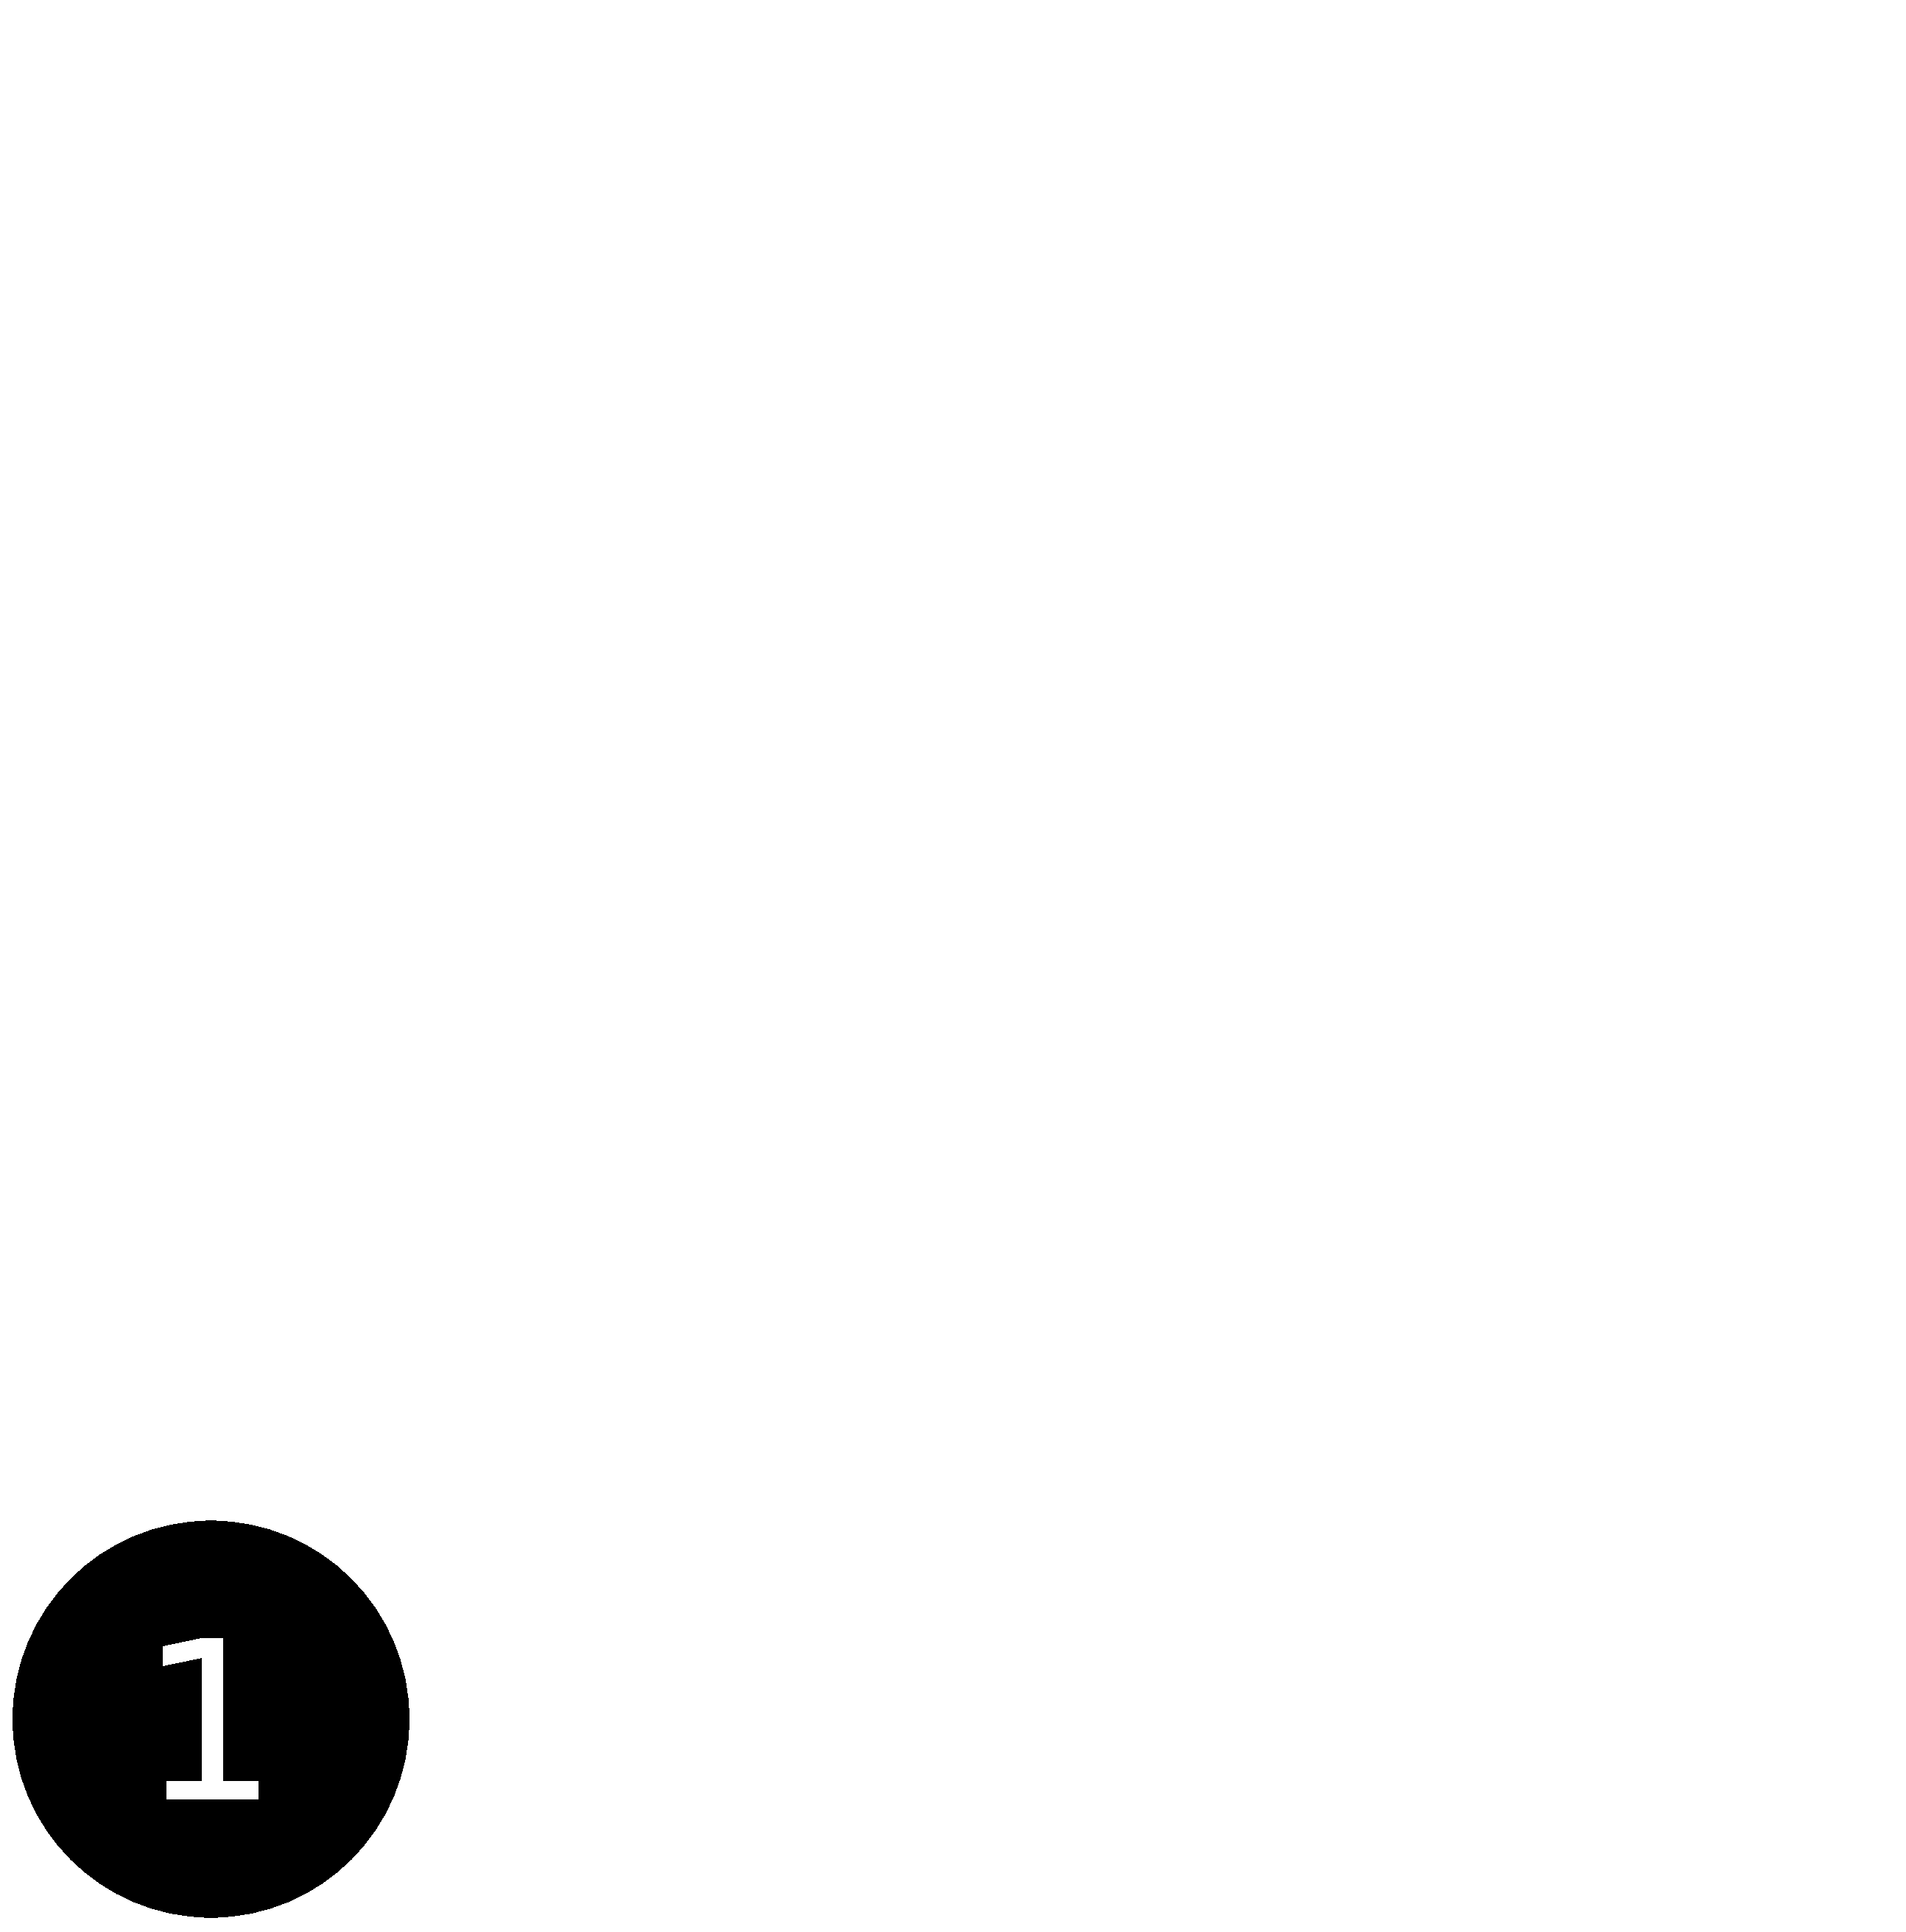
\includegraphics[scale=0.05]{./images/filtration/small/x1.eps}}}%
    \qquad
    \subfloat[$X_1$]{{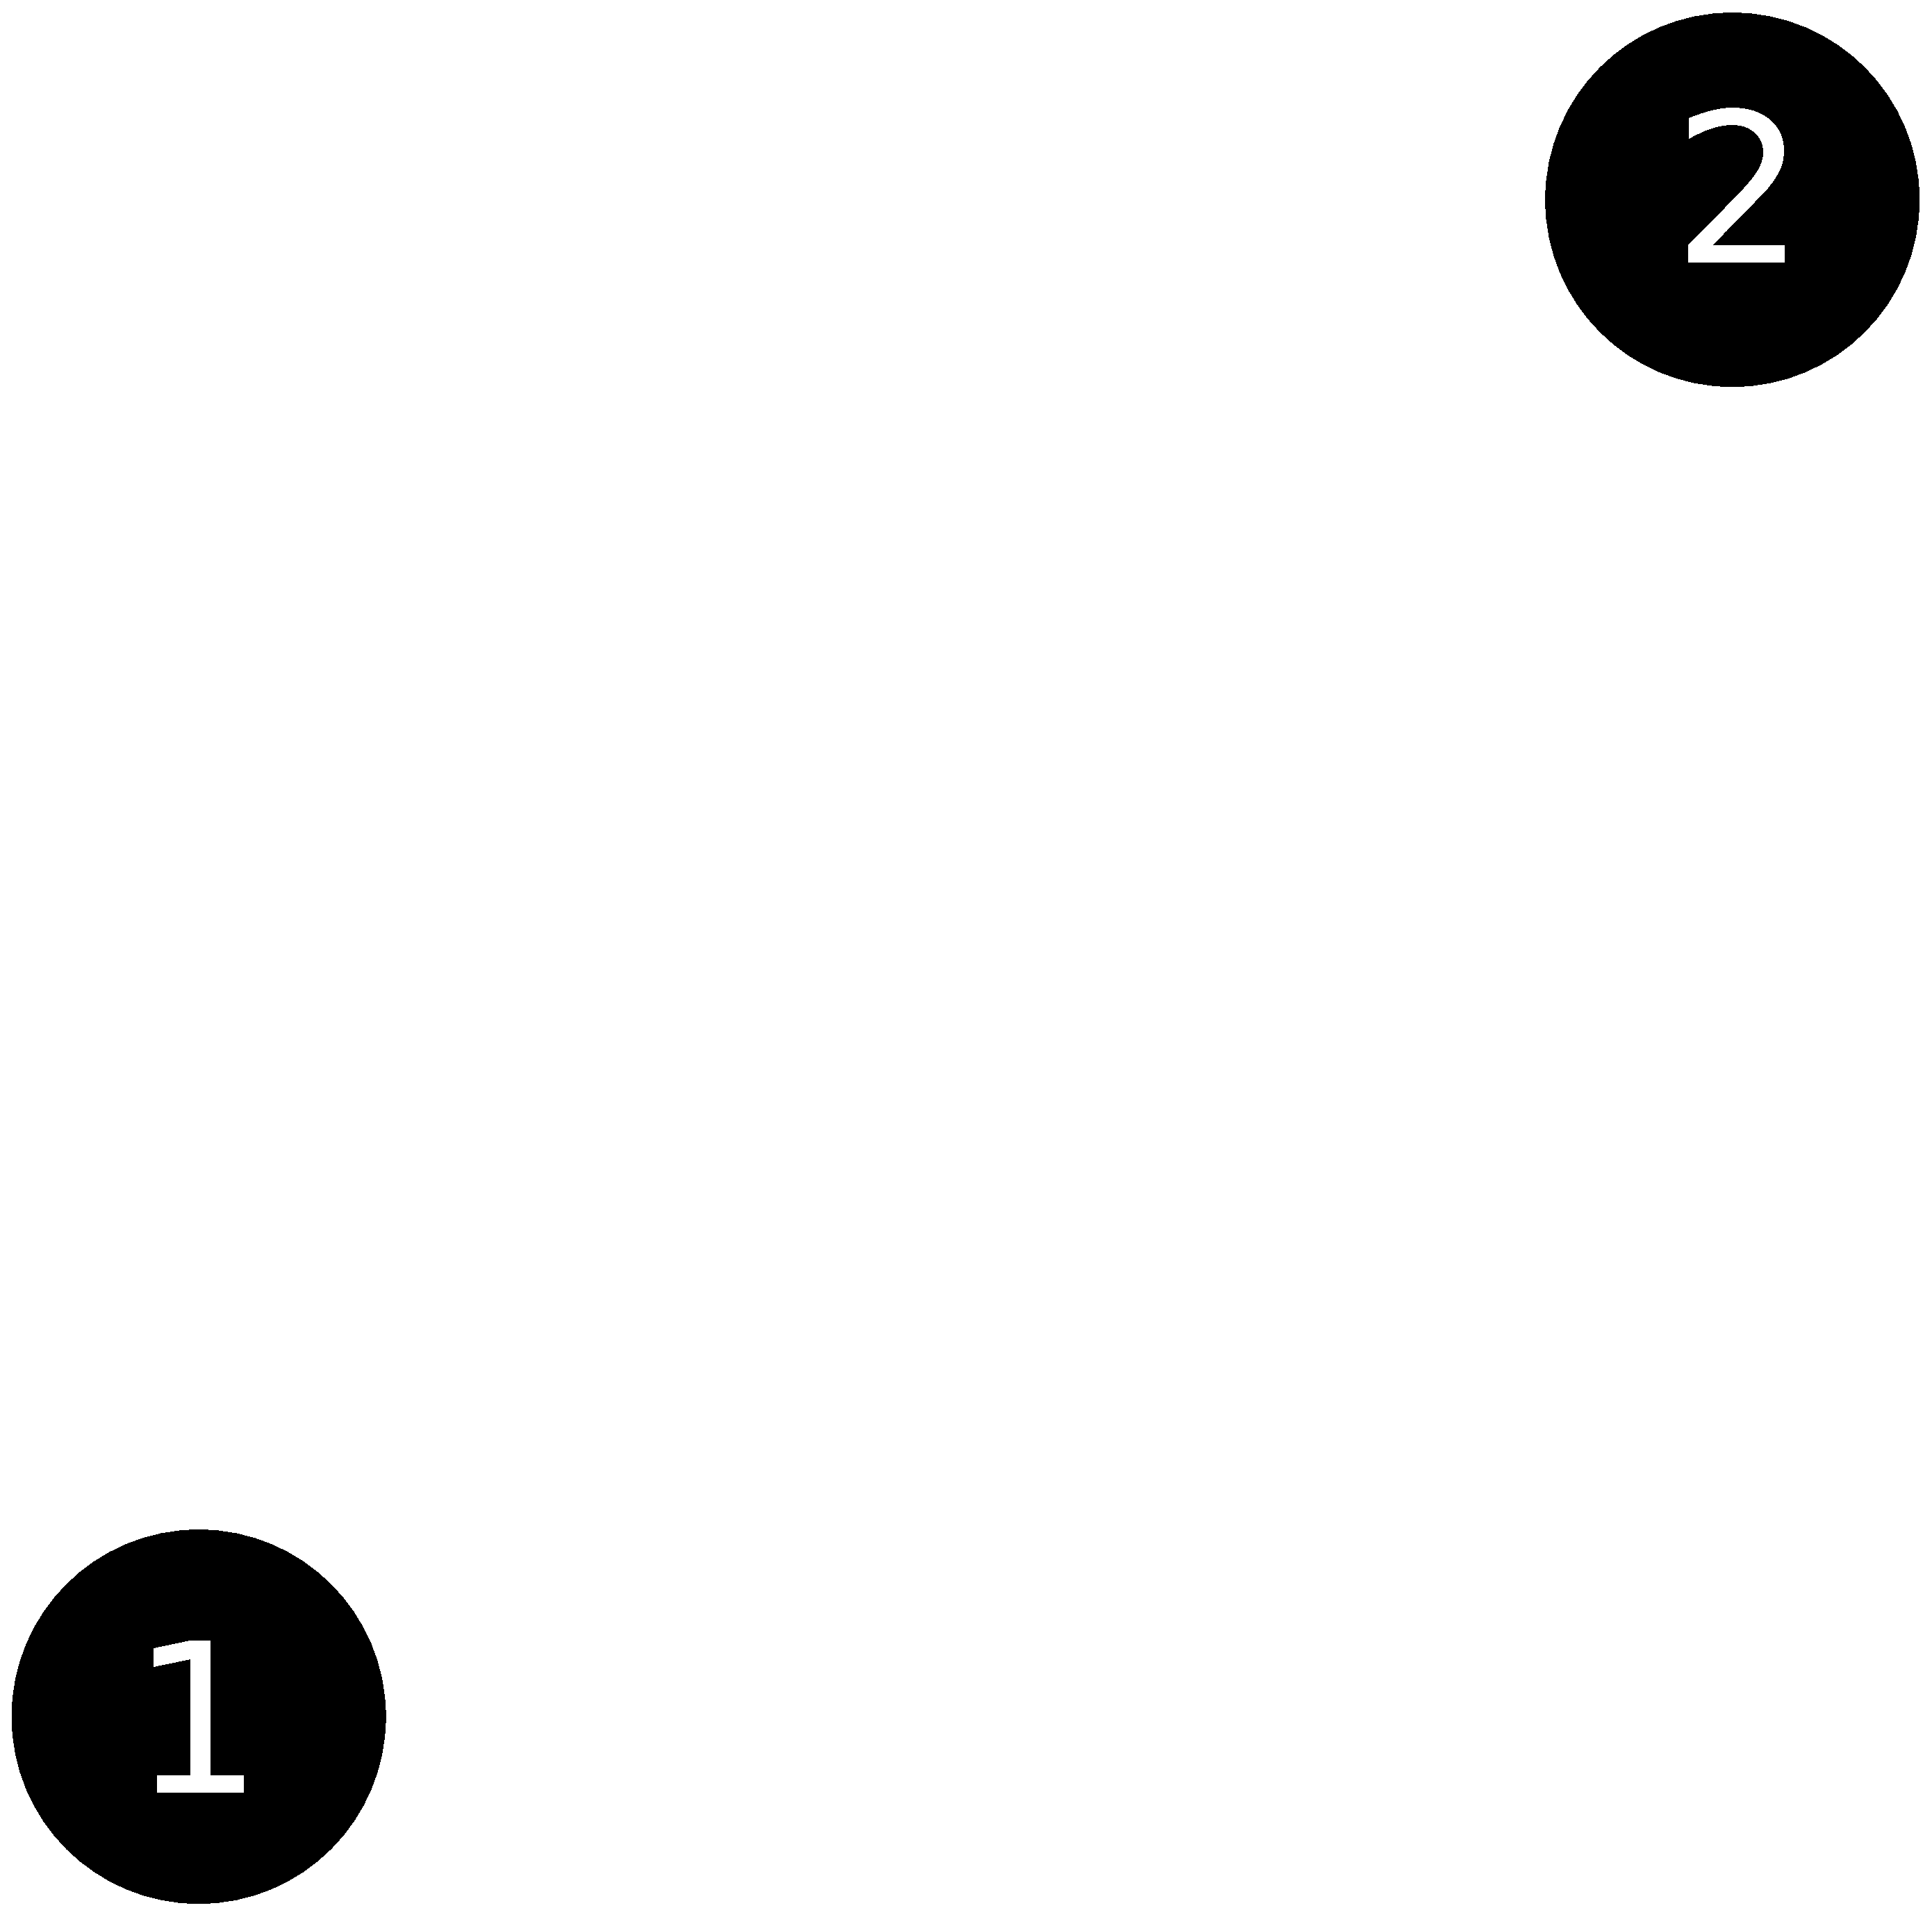
\includegraphics[scale=0.05]{./images/filtration/small/x2.eps}}}%
    \qquad
    \subfloat[$X_2$]{{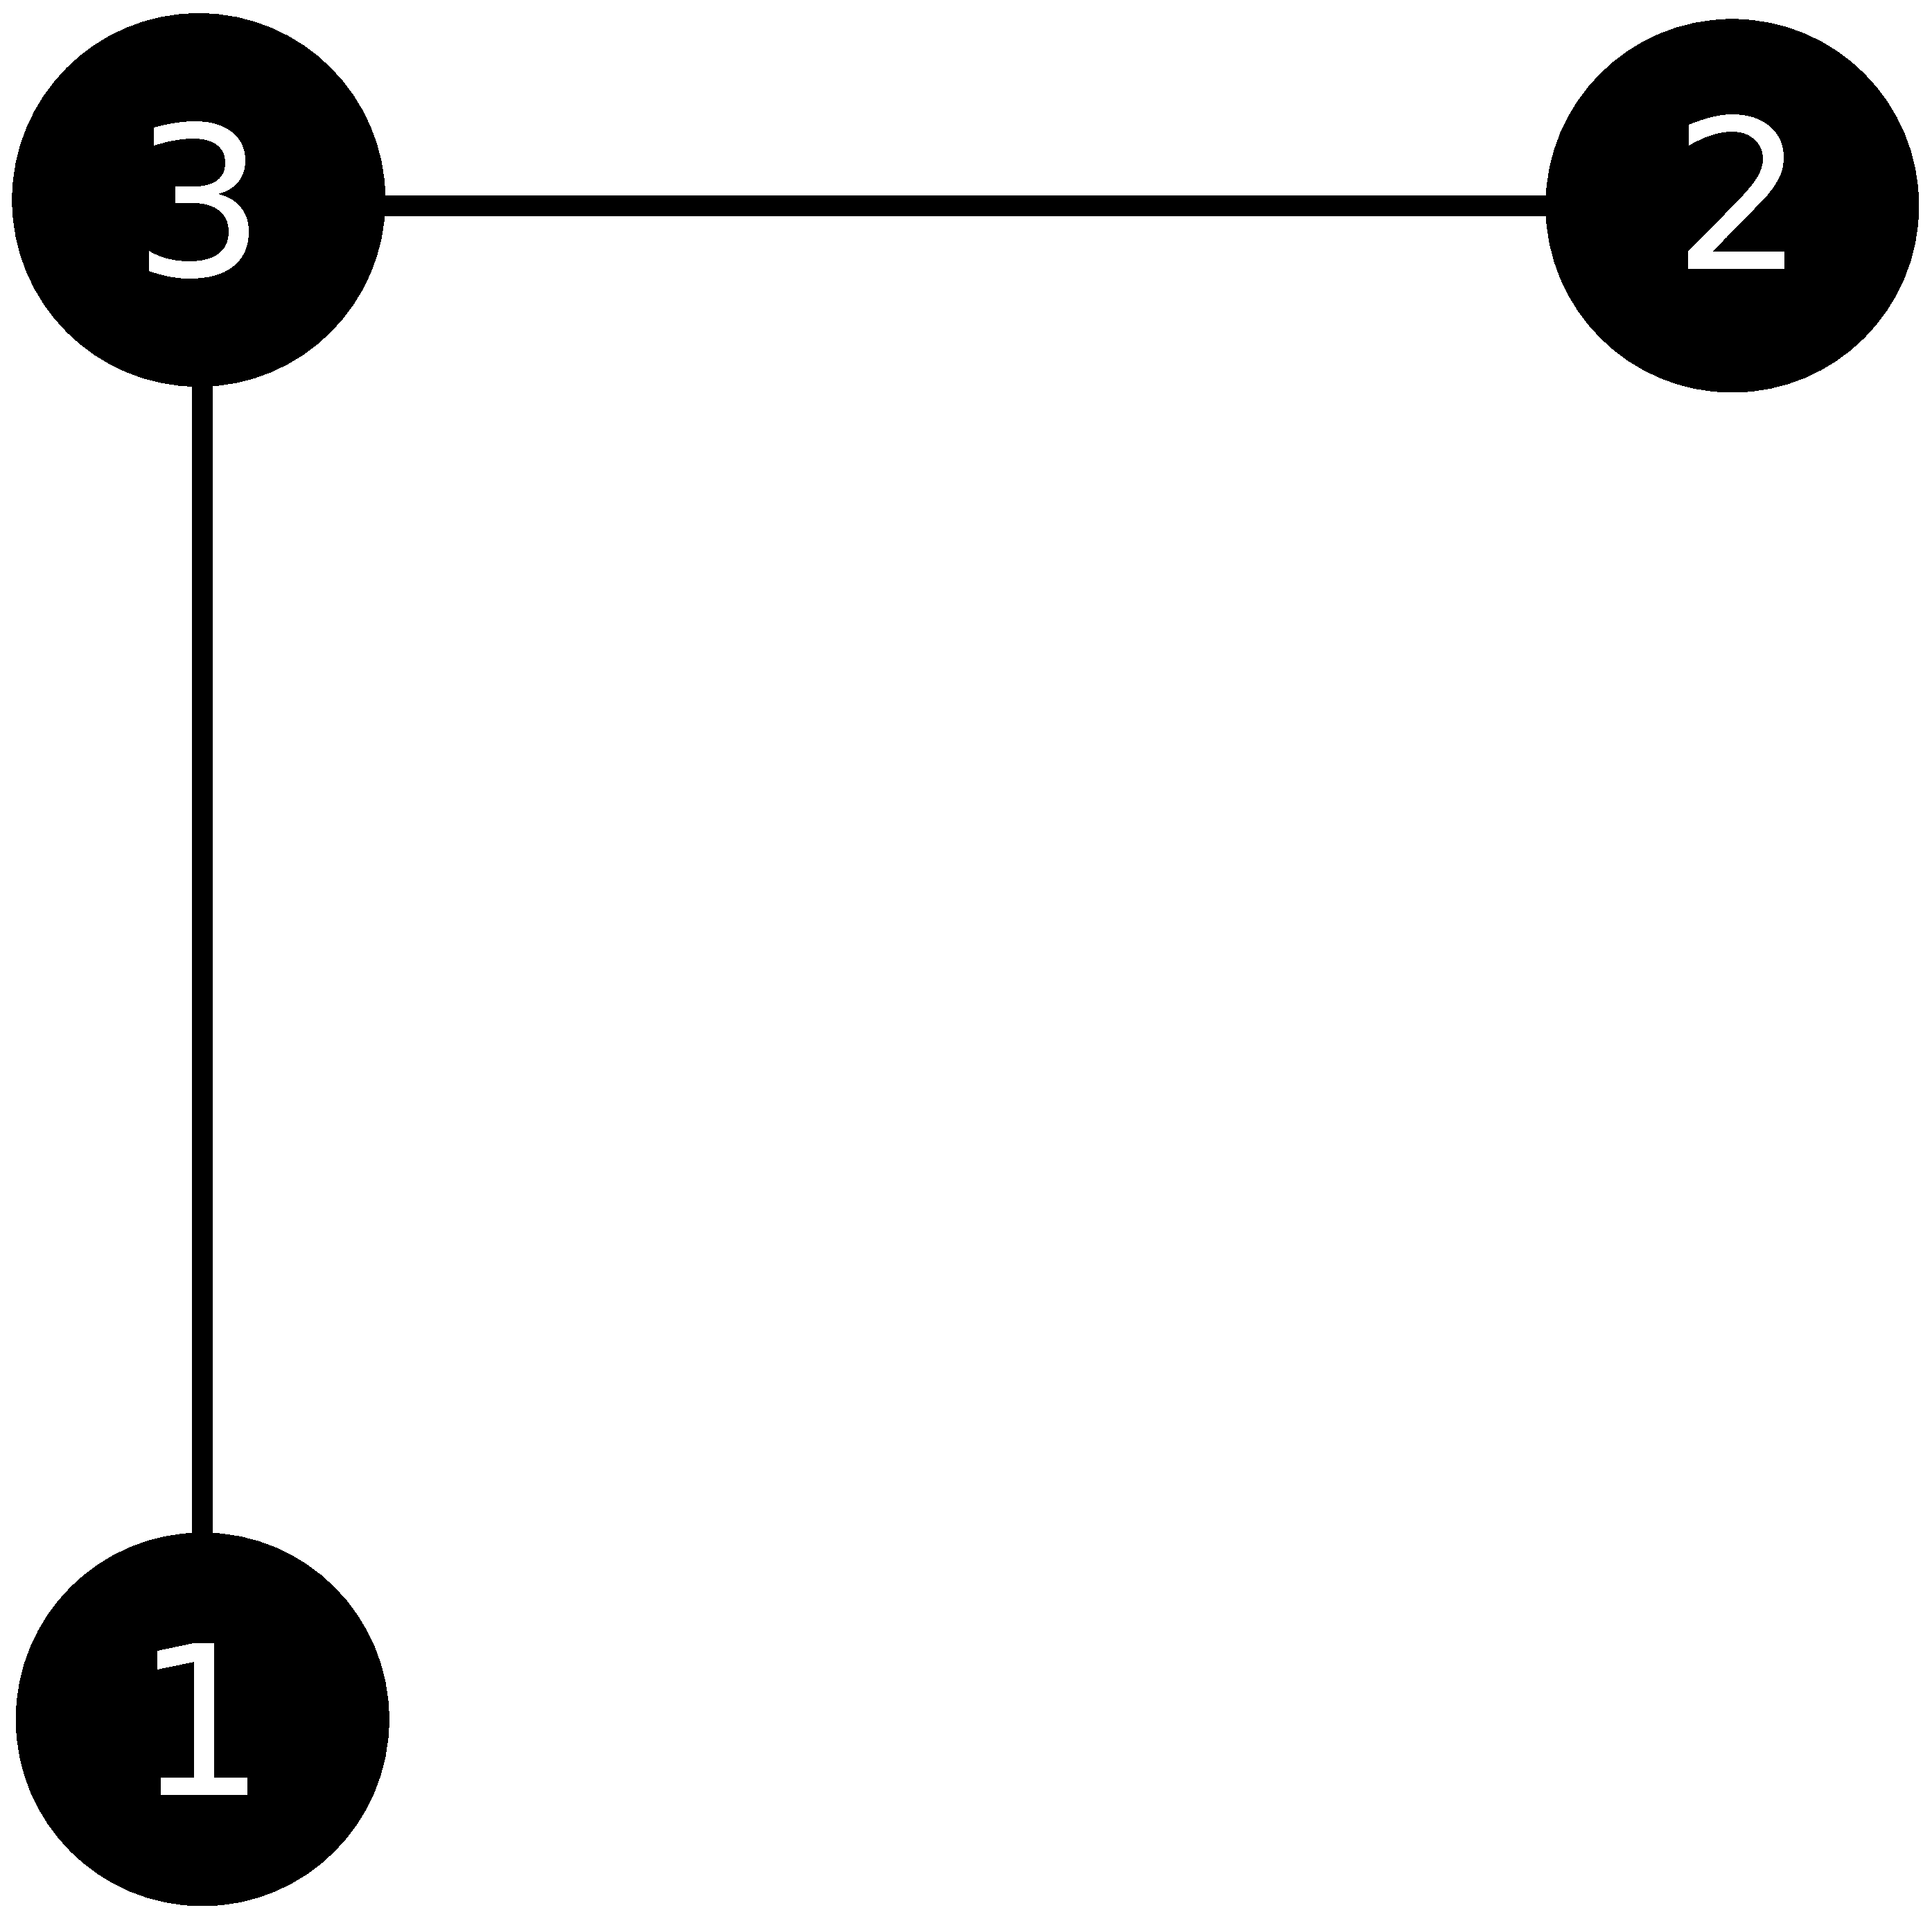
\includegraphics[scale=0.05]{./images/filtration/small/x3.eps}}}%
    \qquad
    \subfloat[$X_3$]{{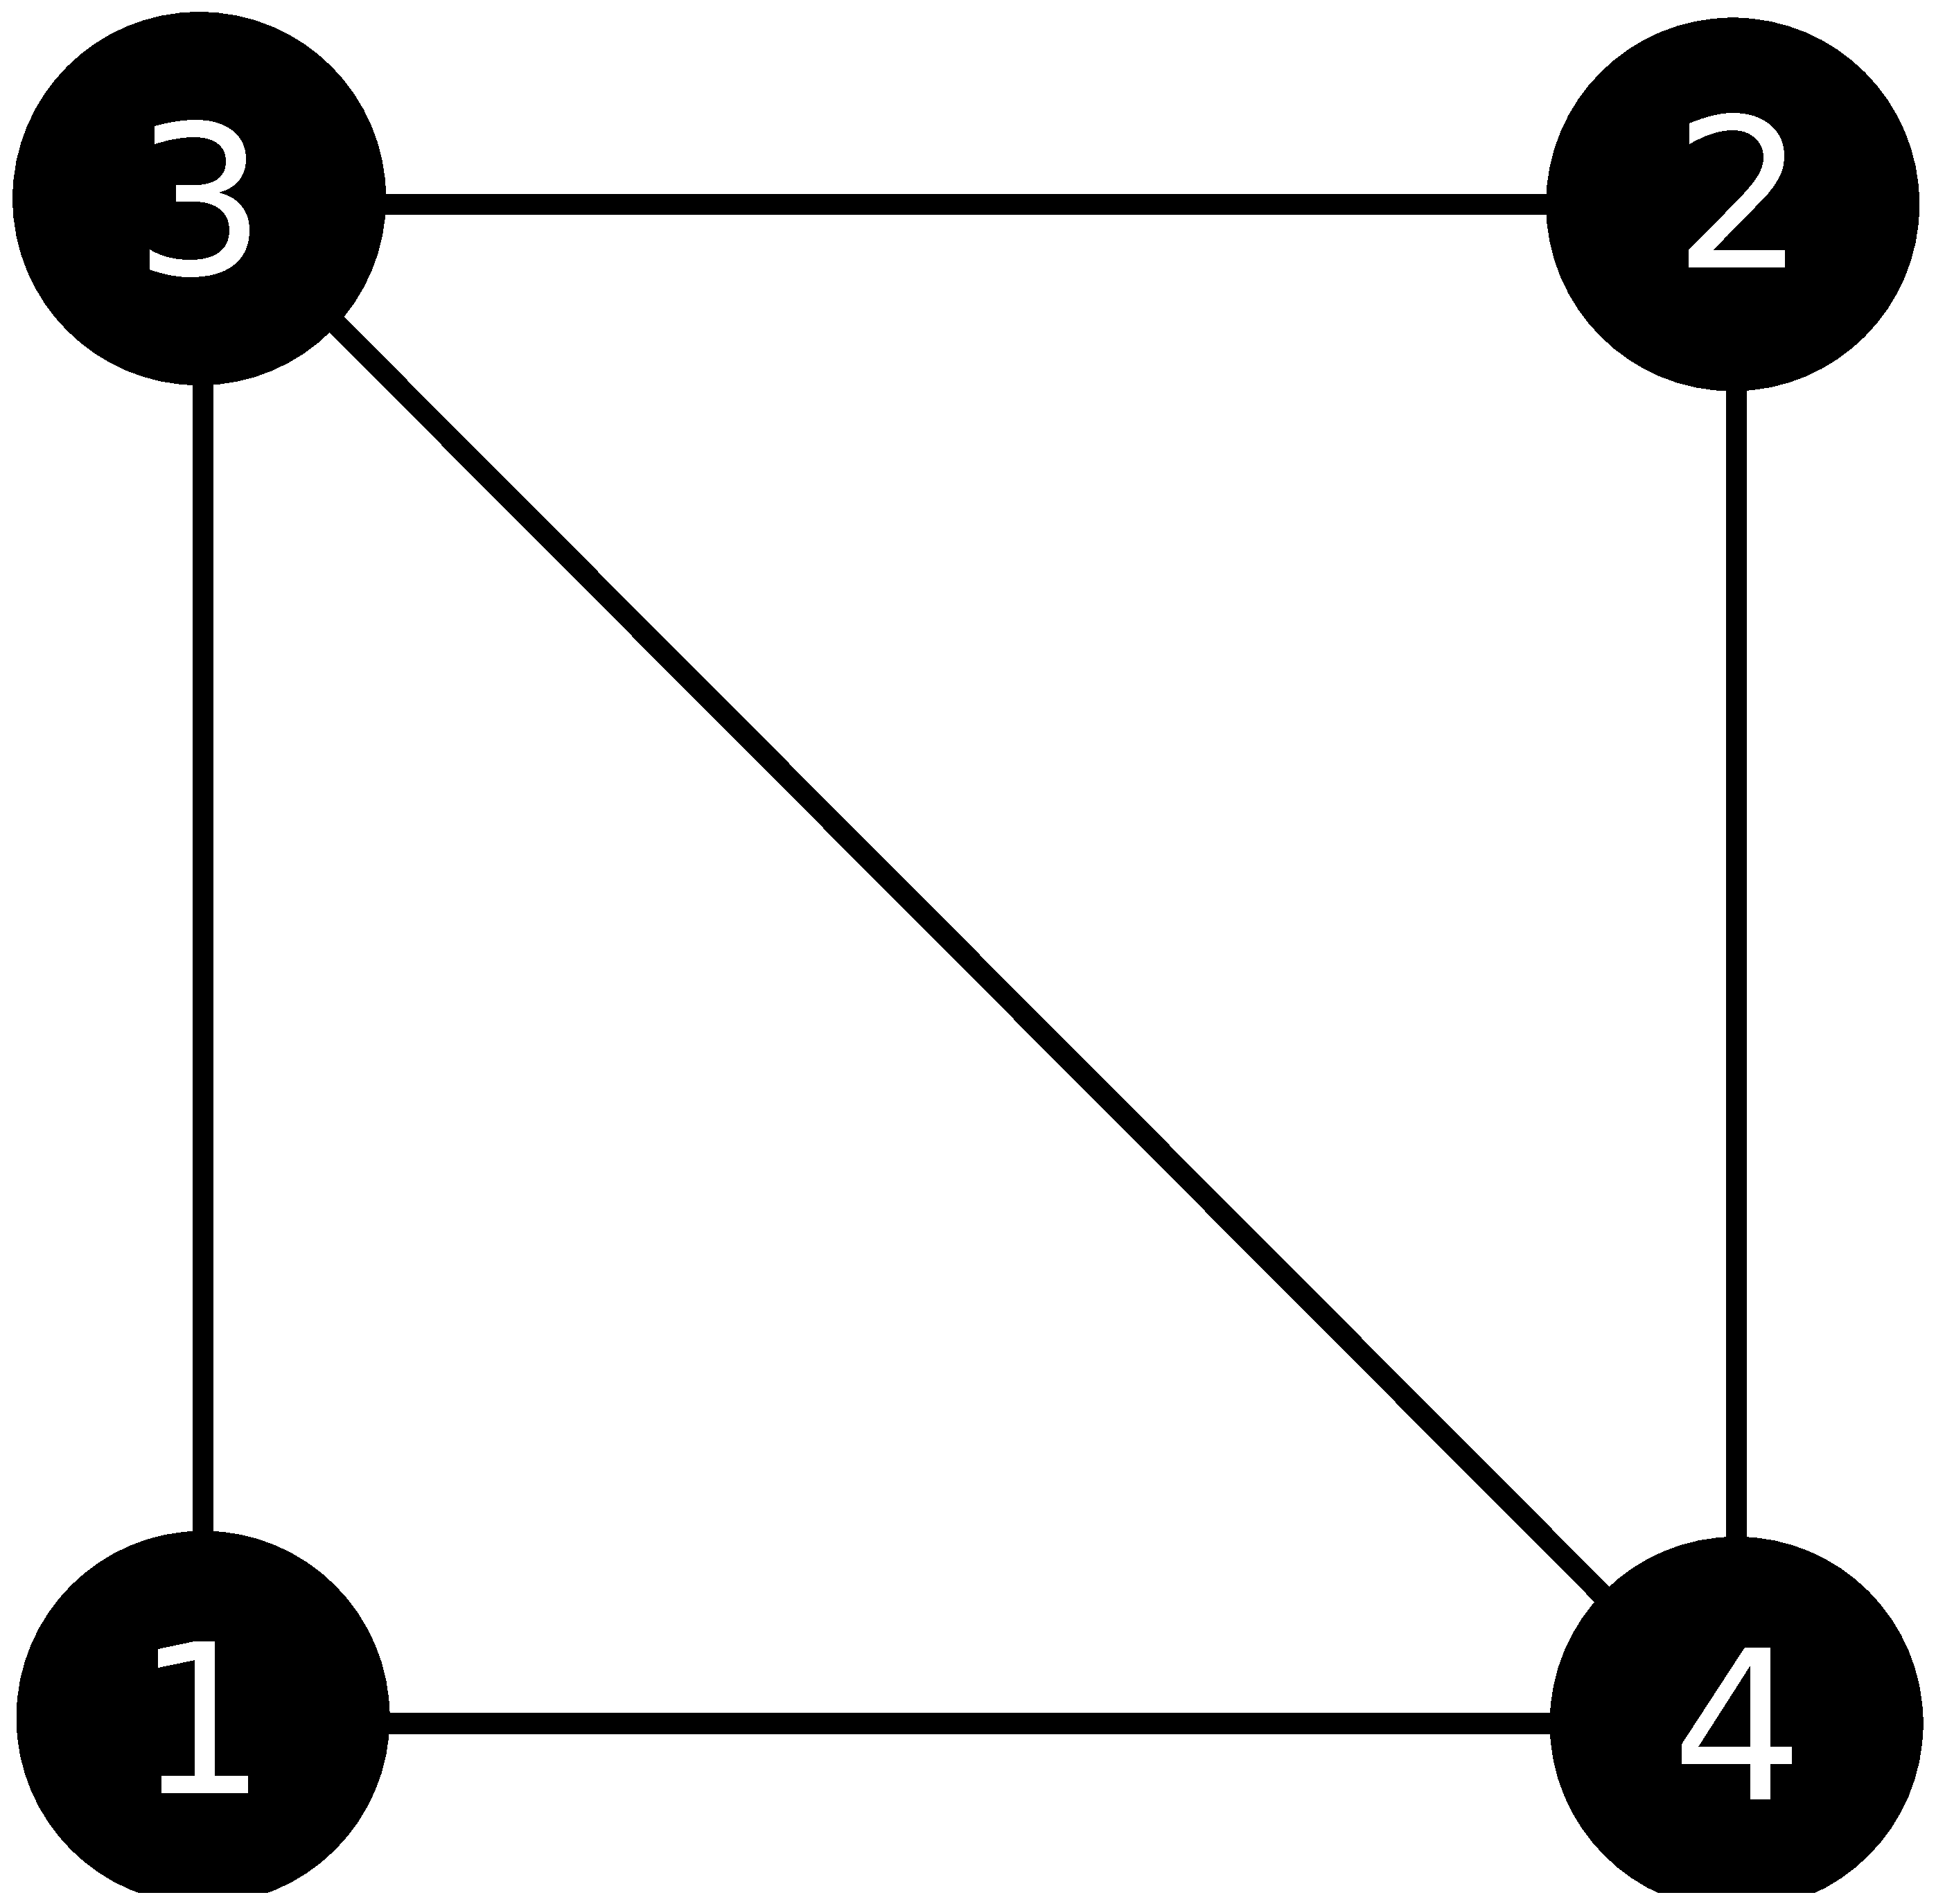
\includegraphics[scale=0.05]{./images/filtration/small/x4.eps}}}%
    \qquad
    \subfloat[$X_4 = X$]{{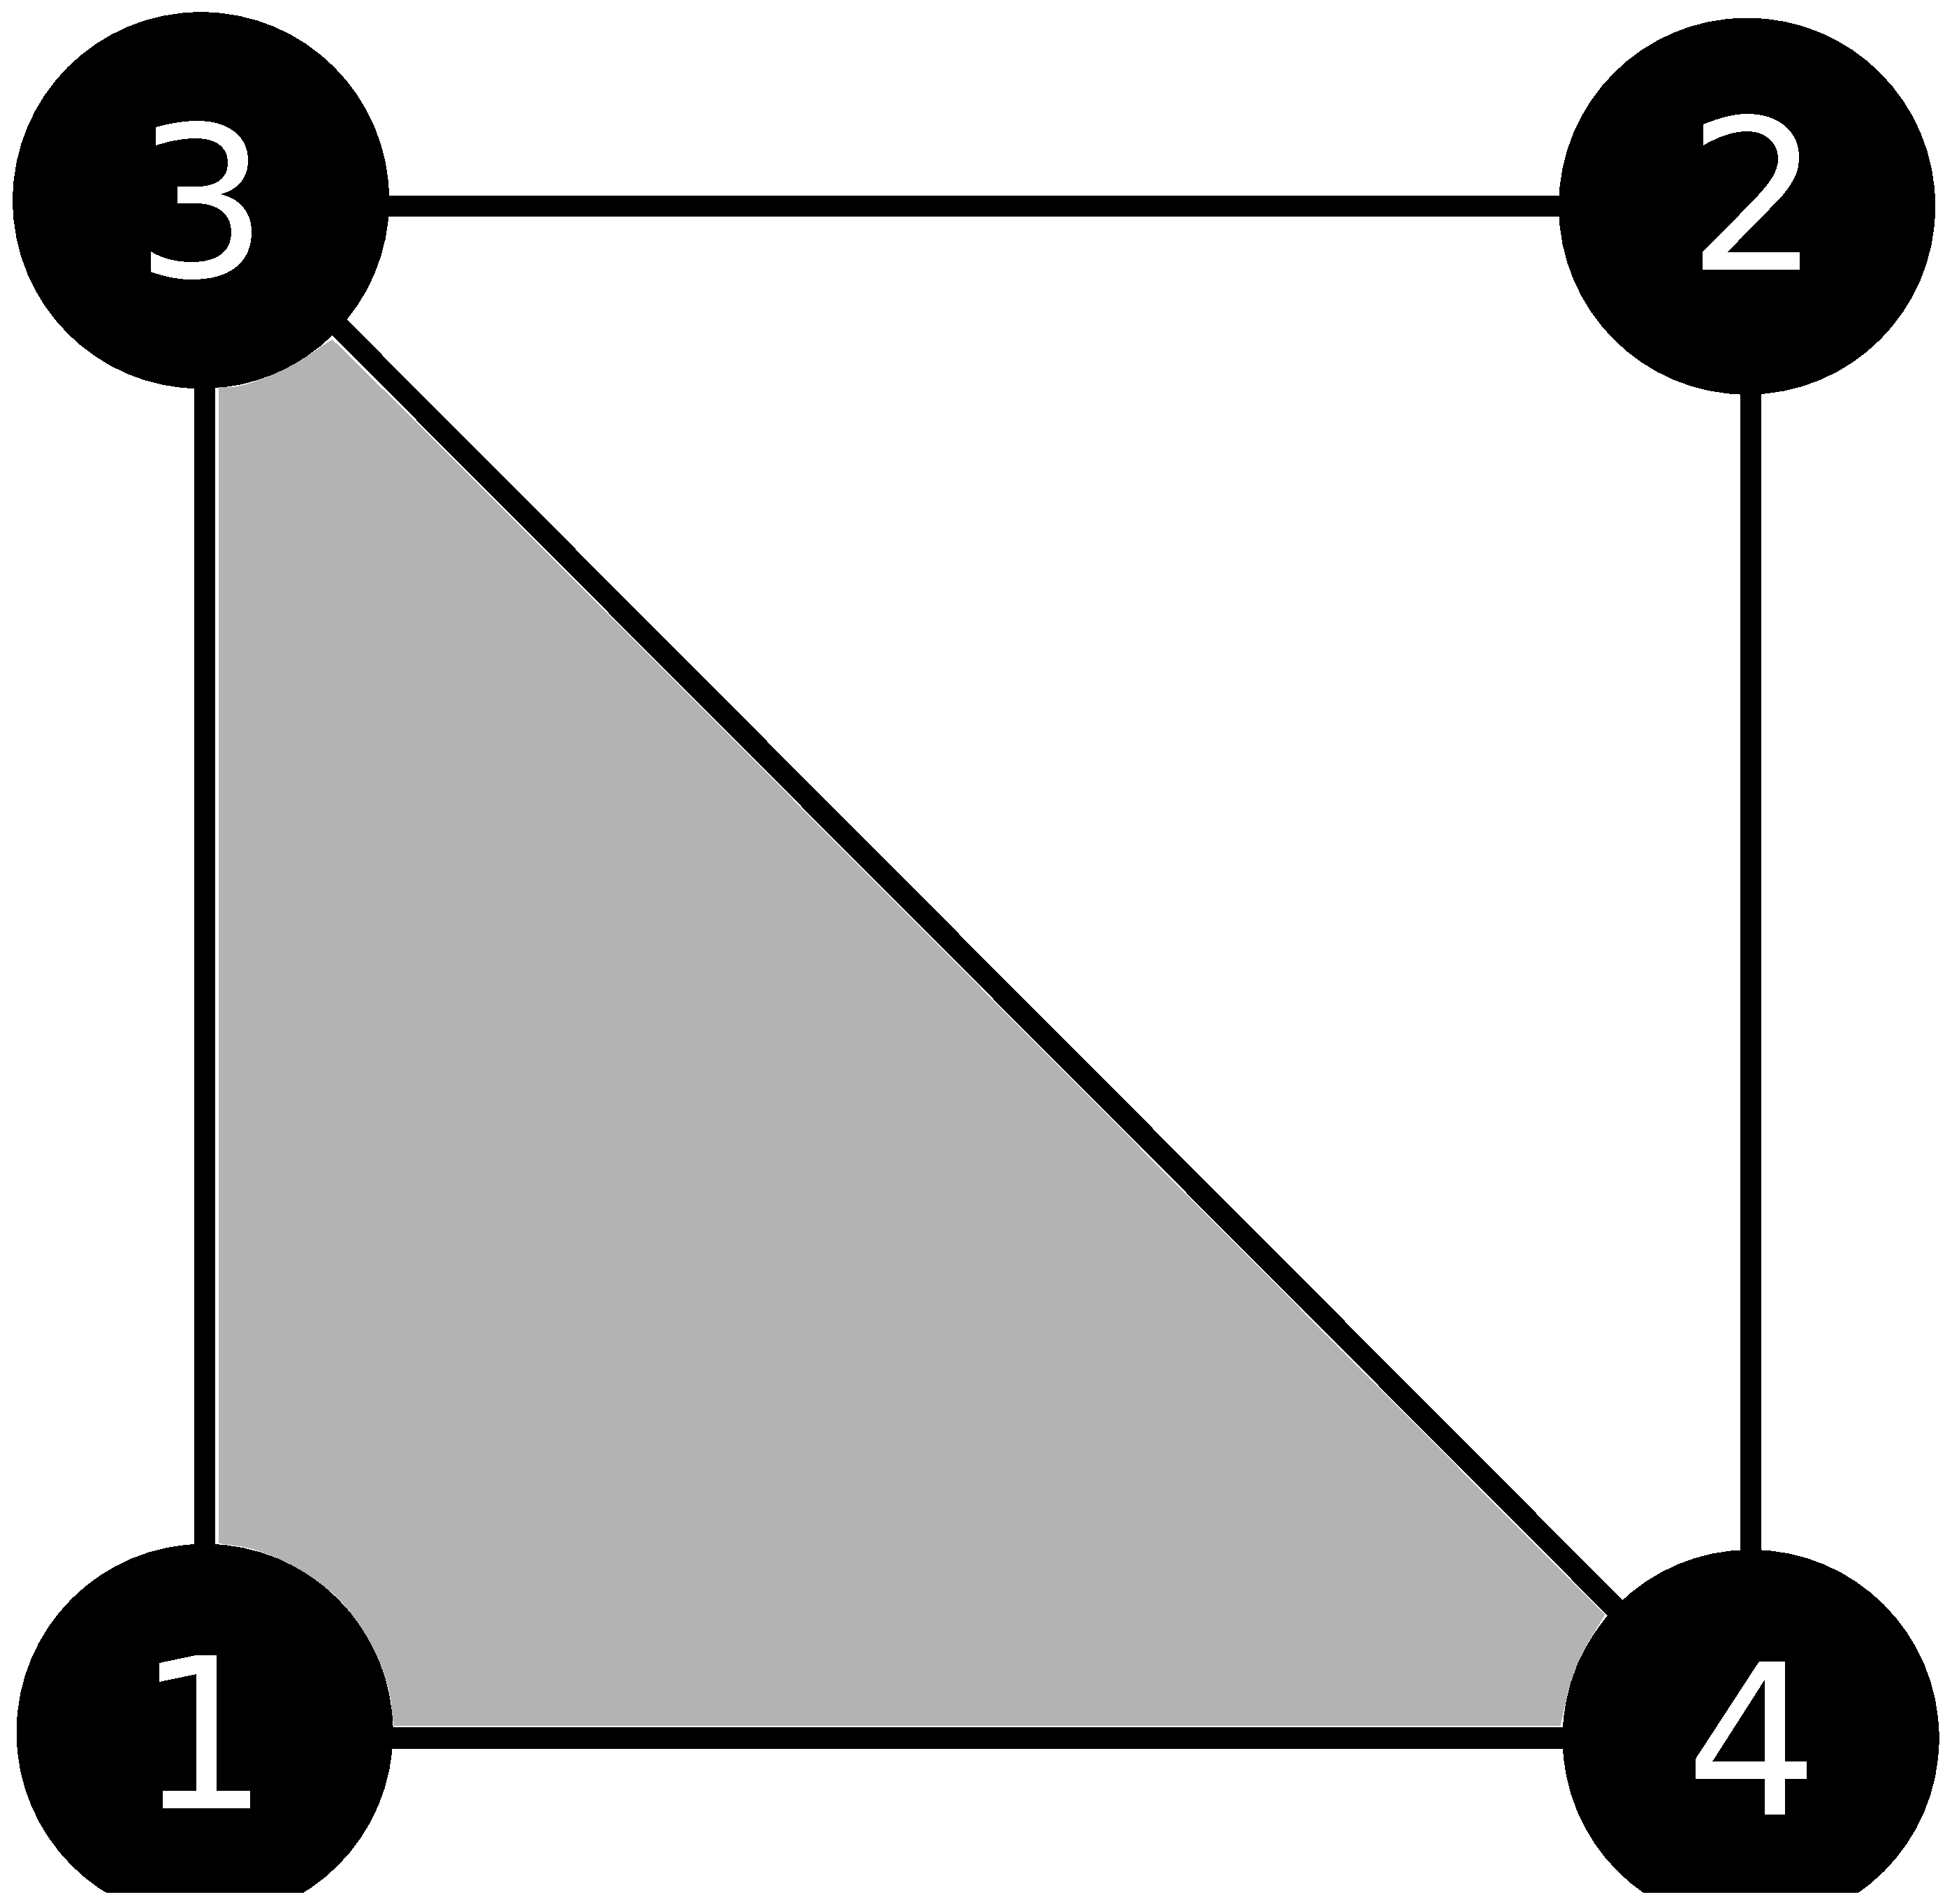
\includegraphics[scale=0.05]{./images/filtration/small/x5.eps}}}%
    \caption{Example of an filtration of a simplicial complex.}%
    \label{fig:example-filtration}%
\end{figure}

% A concrete example of a filtration can be found on Figure \ref{fig:filt-sc}.
%
% \begin{figure}%
%     \centering
%     
\includegraphics[scale=0.085]{./images/chapter4/example-filtration.eps}%
%     \caption{Filtration of a Simplical Complex}%
%     \label{fig:filt-sc}%
% \end{figure}

Another way to think about a filtration is that we start with simplicial complex and iteratively add new simplicies to it. It is customary to call the index of this filtration time to make it more indicative of a process that evolves over time. The key insight in persistent homology comes from realising that we can track individual homology classes in the homology groups of the $X_k$ as we go from one simplical complex to the next. This is made possible by the subset relation between subsequent complexes in the filtration. Since $X_k$ is a subcomplex of $X_{k+1}$ we have inclusion maps $i: X_{k} \to X_{k+1}$ for $k \in \{0, 1, ..., n - 1\}$. Using those inclusion maps we can build the following chain of simplicial complexes.

$$ X_0 \overset{i}{\longrightarrow} X_1 \overset{i}{\longrightarrow} ... \overset{i}{\longrightarrow} X_{n-1} \overset{i}{\longrightarrow} X_n .$$

We have already shown in the previous chapter that inclusion maps induce linear maps between homology groups. By invoking this property we obtain the following sequence of homology groups and maps between them:

$$ H_p(X_0) \overset{i_*}{\longrightarrow} H_p(X_1) \overset{i_*}{\longrightarrow} ... \overset{i_*}{\longrightarrow} H_p(X_{n-1}) \overset{i_*}{\longrightarrow} H_p(X_n) $$
for all $p \in \{0, 1, 2, ...\}$. The induced linear maps encode the information about the topological changes in the homology of consecutive complexes in the filtration. We will introduce the following terminology to help us interpret this information \cite{elementary-applied-topology}:

\begin{itemize}
    \item A homology class is \textbf{born} if it is not in the image of the homology group of the previous complex in the filtration under $i_*$.
    \item A homology class \textbf{dies} if its image under $i_*$ is the zero element or it merges with an older class.
    \item A homology class \textbf{persists} if its image under $i_*$ is not the zero element and it does not merge with an older class.
\end{itemize}

Let us now expand on the case when two classes merge in a filtration. Suppose that $[\alpha] \ne [\beta]$ are two homology classes of some $H_p(X_i)$ such that $i_*([\alpha]) = i_*([\beta])$ in $H_p(X_{i+1})$ because of the introduction of a new boundary. For example the classes $[0]$ and $[1]$ in $H_0(X_1)$ are not equivalent. They represent two distinct connected components. By introducing the edge $01$ in $X_1$ they become one connected component and $[0] = [1]$ in $H_0(X_2)$. We must choose which one of the classes dies and which one of them persists. It does not matter what we choose as long as we commit to the choice in the future.

In order to be consistent in choosing we will apply the Elder Rule \cite[p.~150]{comp-topo}. According to the elder rule the class whose birth time is smaller will persist and the other one will die. In the case of merging multiple classes all will die except for the oldest. In the example where $[0] = [1]$ in $H_0(X_2)$ we will pick $[0]$ as the representative of the homology class because it is older and say that $[1]$ dies at time $2$ because it merges with $[0]$.

Using the language of birth and death we can define the persistence of a homology class. Let $\alpha$ be a homology class that is born in $X_i$ and dies in $X_j$. We call the difference $j - i$ the persistence of $\alpha$. Some classes however do not have a defined death time. These are the classes of the final complex in the filtration. We will call those classes essential and set their persistence to $\infty$. Classes that have persisted for a large number of timesteps are deemed significant. Ephemeral classes on the other hand are not. Such classes are often considered to correspond to statistical noise or sampling error.

One way to visualise persistent homology is by producing the so called persistence pairs and plotting them. A persistence pair $(t_1, t_2)$ of a homology class $\alpha$ is a pairing of two timestamps - the birth and death time of $\alpha$. The essential classes are the exception to this rule. A persistence pair of an essential class is formed as $(t, \infty)$ where their birth time is $t$ and we set their death time to $\infty$ due to the lack of one.

Persistence pairs are visualised by plotting them as points in the plane. This is called a persistence diagram. We denote the essential classes as triangles above the last simplex in the filtration and other classes as circles (Figure \ref{fig:ph-viz} a, b). We can see that there are two pairs in the 0th persistent homology of the filtration on Figure \ref{fig:example-filtration}. The first pair is $(1, 2)$ and it corresponds to the birth of the second connected component in time $1$ and its death in time $2$ where it merges with the first connected component. The second pair $(0, \infty)$ is an essential class that corresponds to the single connected component of $X_0$ that persists until the end of the filtration at $X_4$.

In the 1st persistent homology we have two pairs. One is $(3, 4)$ and the other is $(3, \infty)$. These correspond to two 1-cycles that are born at time $3$. Those are $13 + 14 + 34$ and $23 + 24 + 34$. At time $4$ the cycle $13 + 14 + 34$ becomes trivial in $H_1(X_4)$ because we add the boundary $234$. The cycle $23 + 24 + 34$ however persists in $H_1(X_4)$ and therefore corresponds to the pair $(3, \infty)$.

Another way to visualize persistent homology is via a barcode diagram \cite{barcodes}. A barcode diagram is a graphical representation of the persistent homology as a collection of horizontal line segments in the plane. The horizontal axis corresponds to the current homology group and the vertical axis corresponds to an arbitrarily chosen basis for the current homology group. A line is drawn between two basis elements $[\alpha] \in H_k(X_t)$ and $[\beta] \in H_k(X_{t+1})$ whenever $i_*[\alpha] = [\beta]$. A line is cut short when a basis element in $H_k(X_t)$ dies upon entering $H_k(X_{t+1})$. The persistent pairs correspond uniquely to lines in the barcode diagram. If there is a persistence pair $(t_1, t_2)$ then we draw a line from $t_1$ and cut it off at $t_2$. For example the barcode diagram for the persistent homology of the filtration on Figure \ref{fig:example-filtration} is depicted on Figure \ref{fig:ph-viz} c).

\begin{figure}[h]%
    \centering
    \subfloat[Persistence pairs in $H_0$.]{{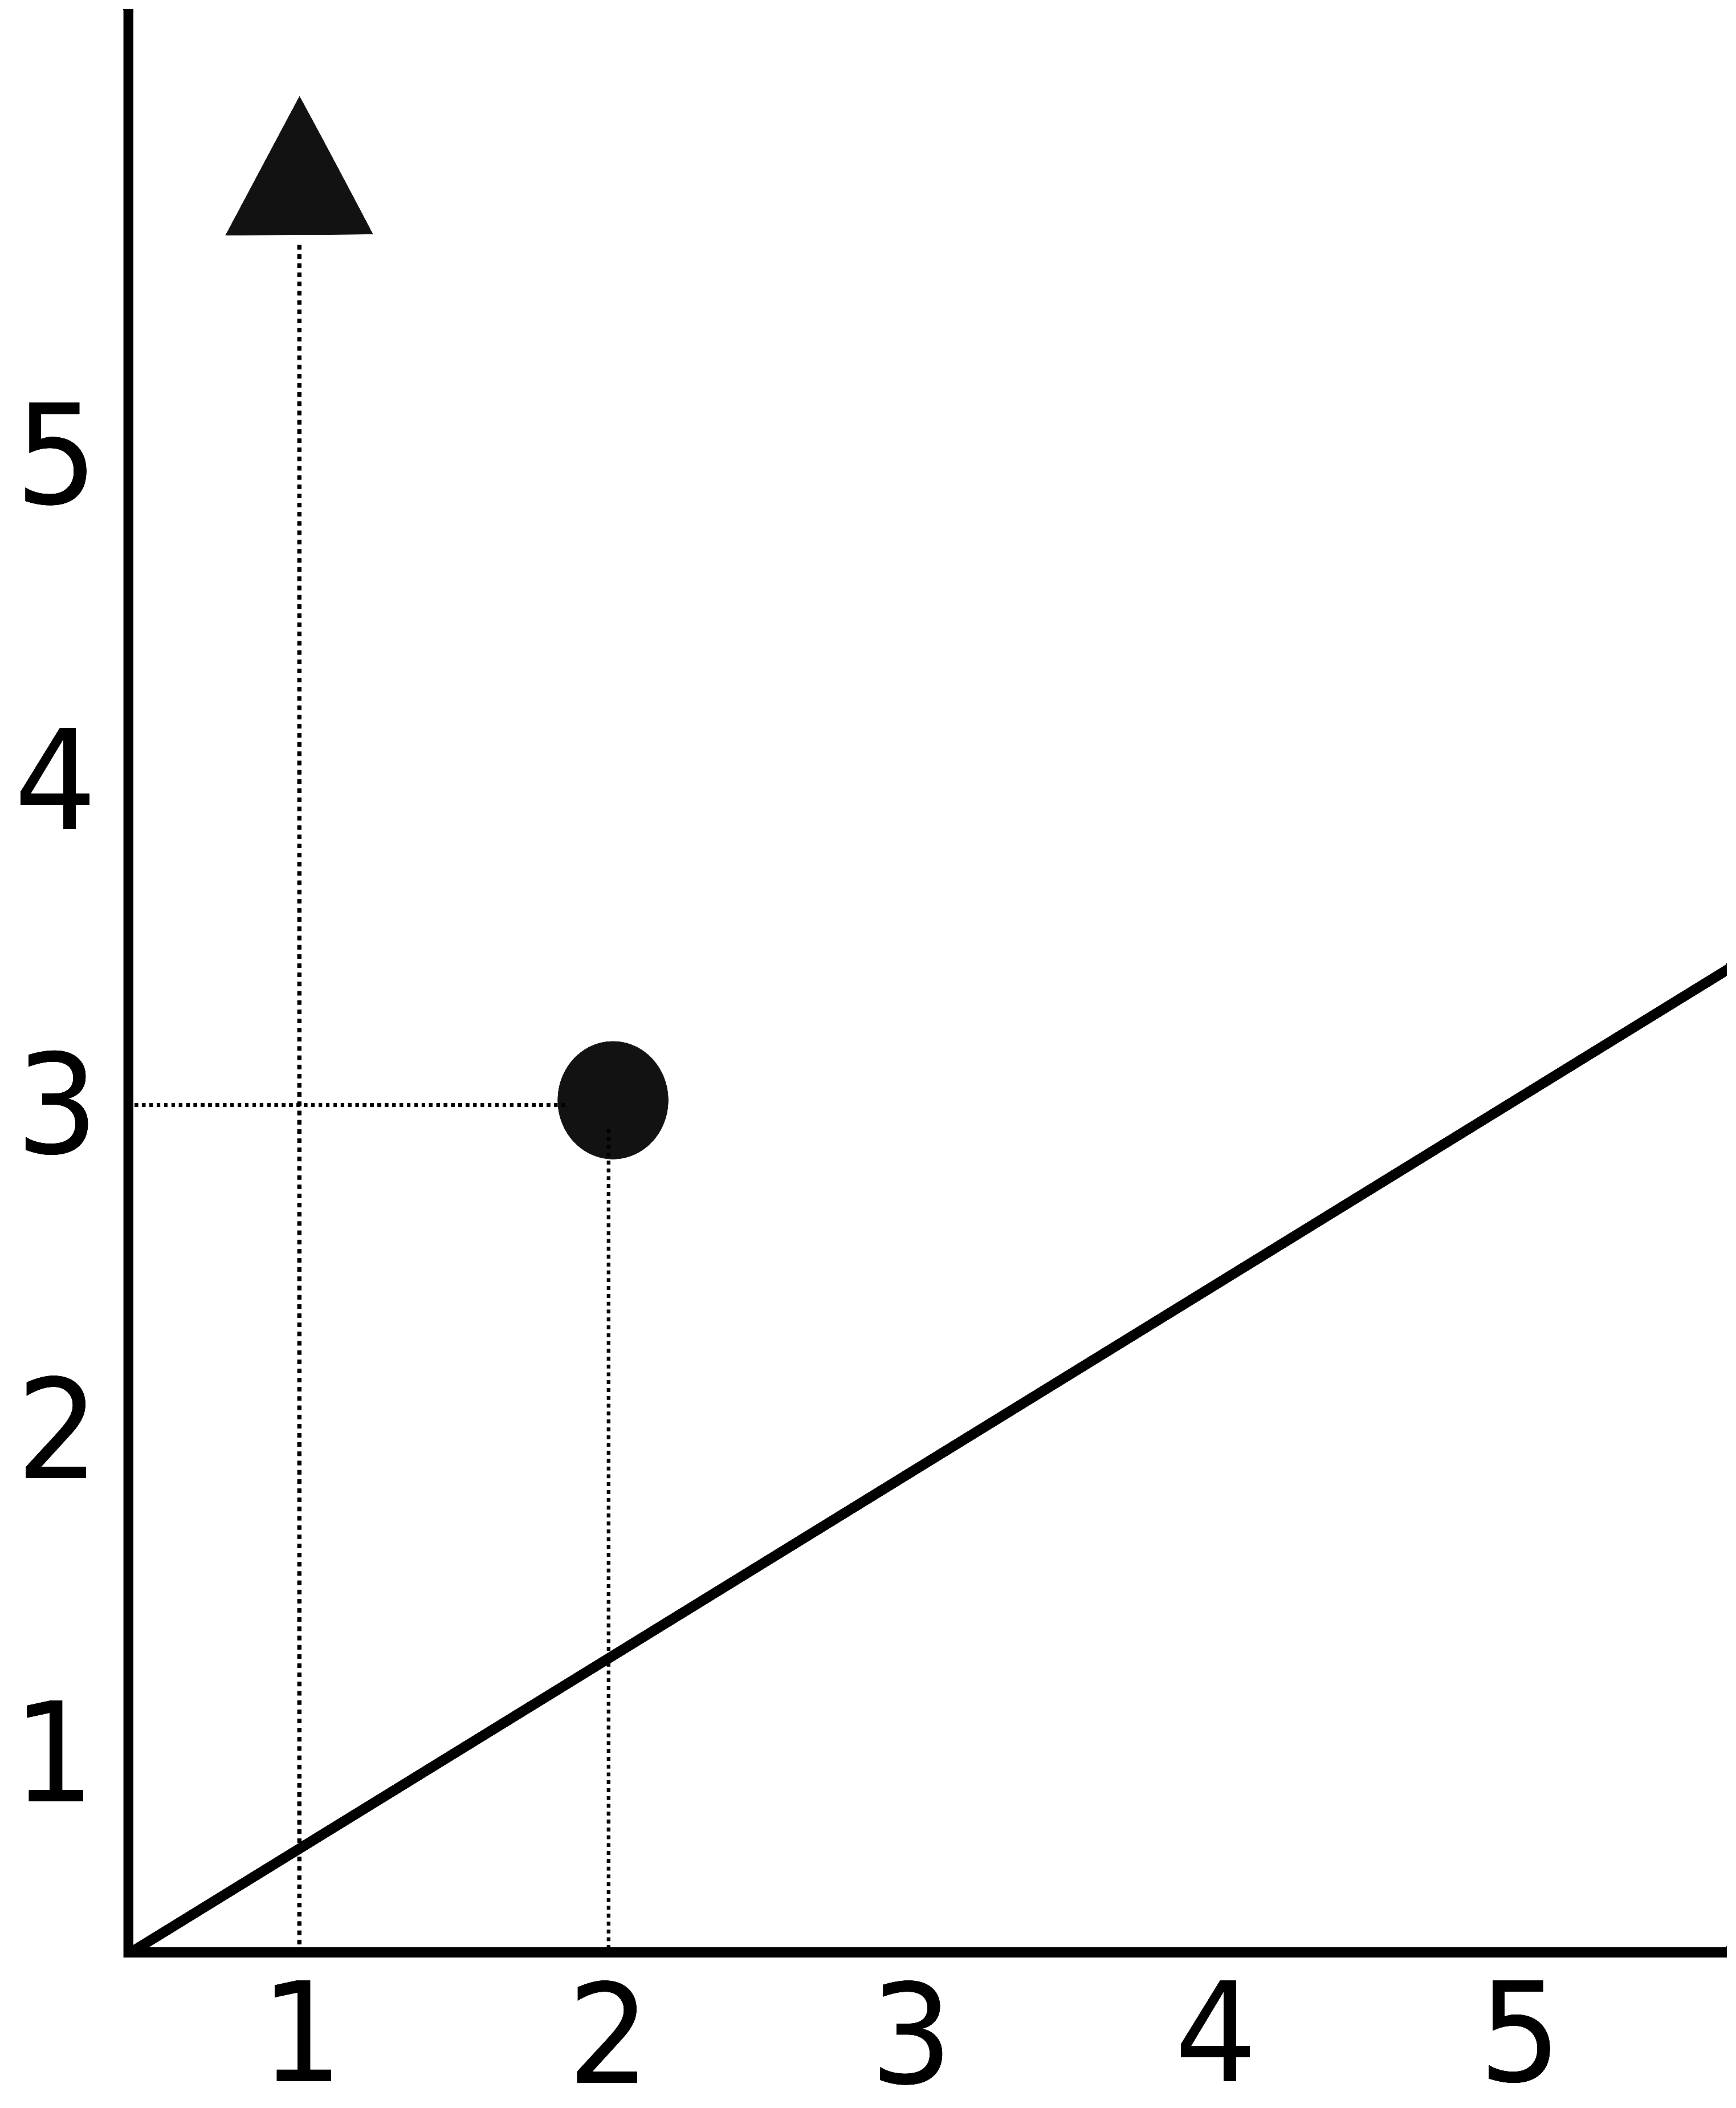
\includegraphics[scale=0.07]{./images/filtration/small/diagram-h0.eps}}}%
    \qquad
    \subfloat[Persistence pairs in $H_1$.]{{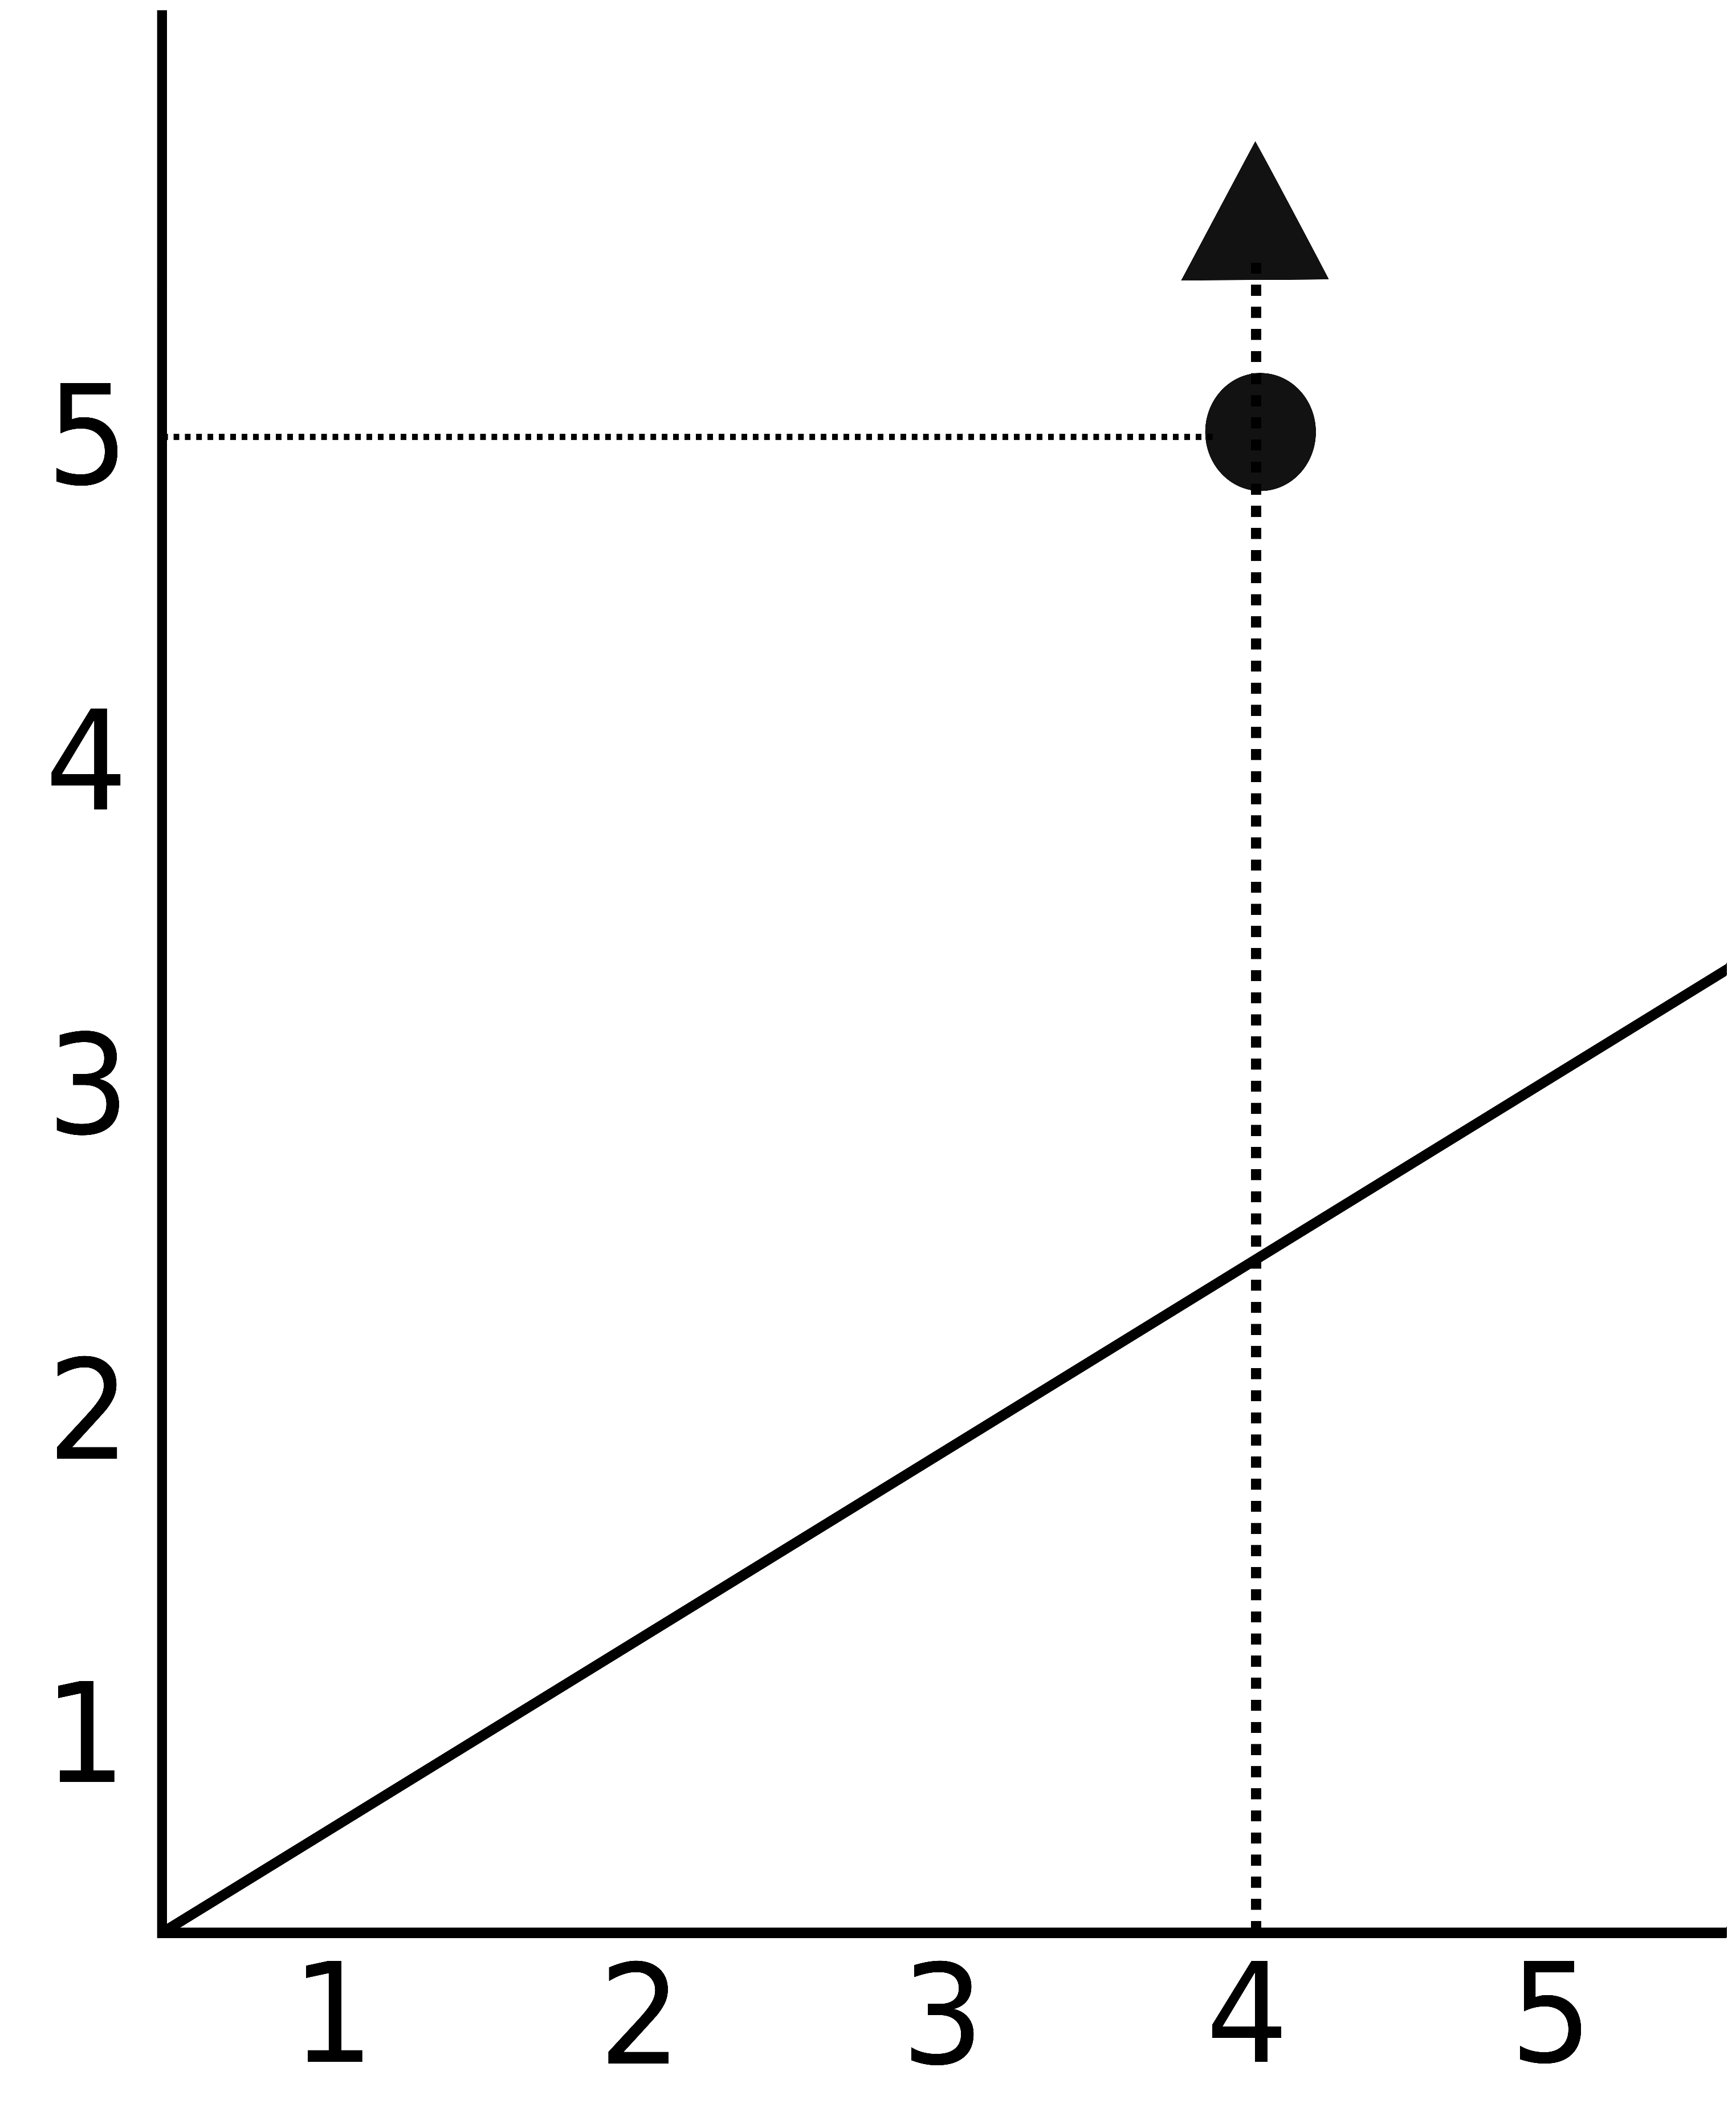
\includegraphics[scale=0.07]{./images/filtration/small/diagram-h1.eps}}}%
    \subfloat[Barcode Diagram.]{{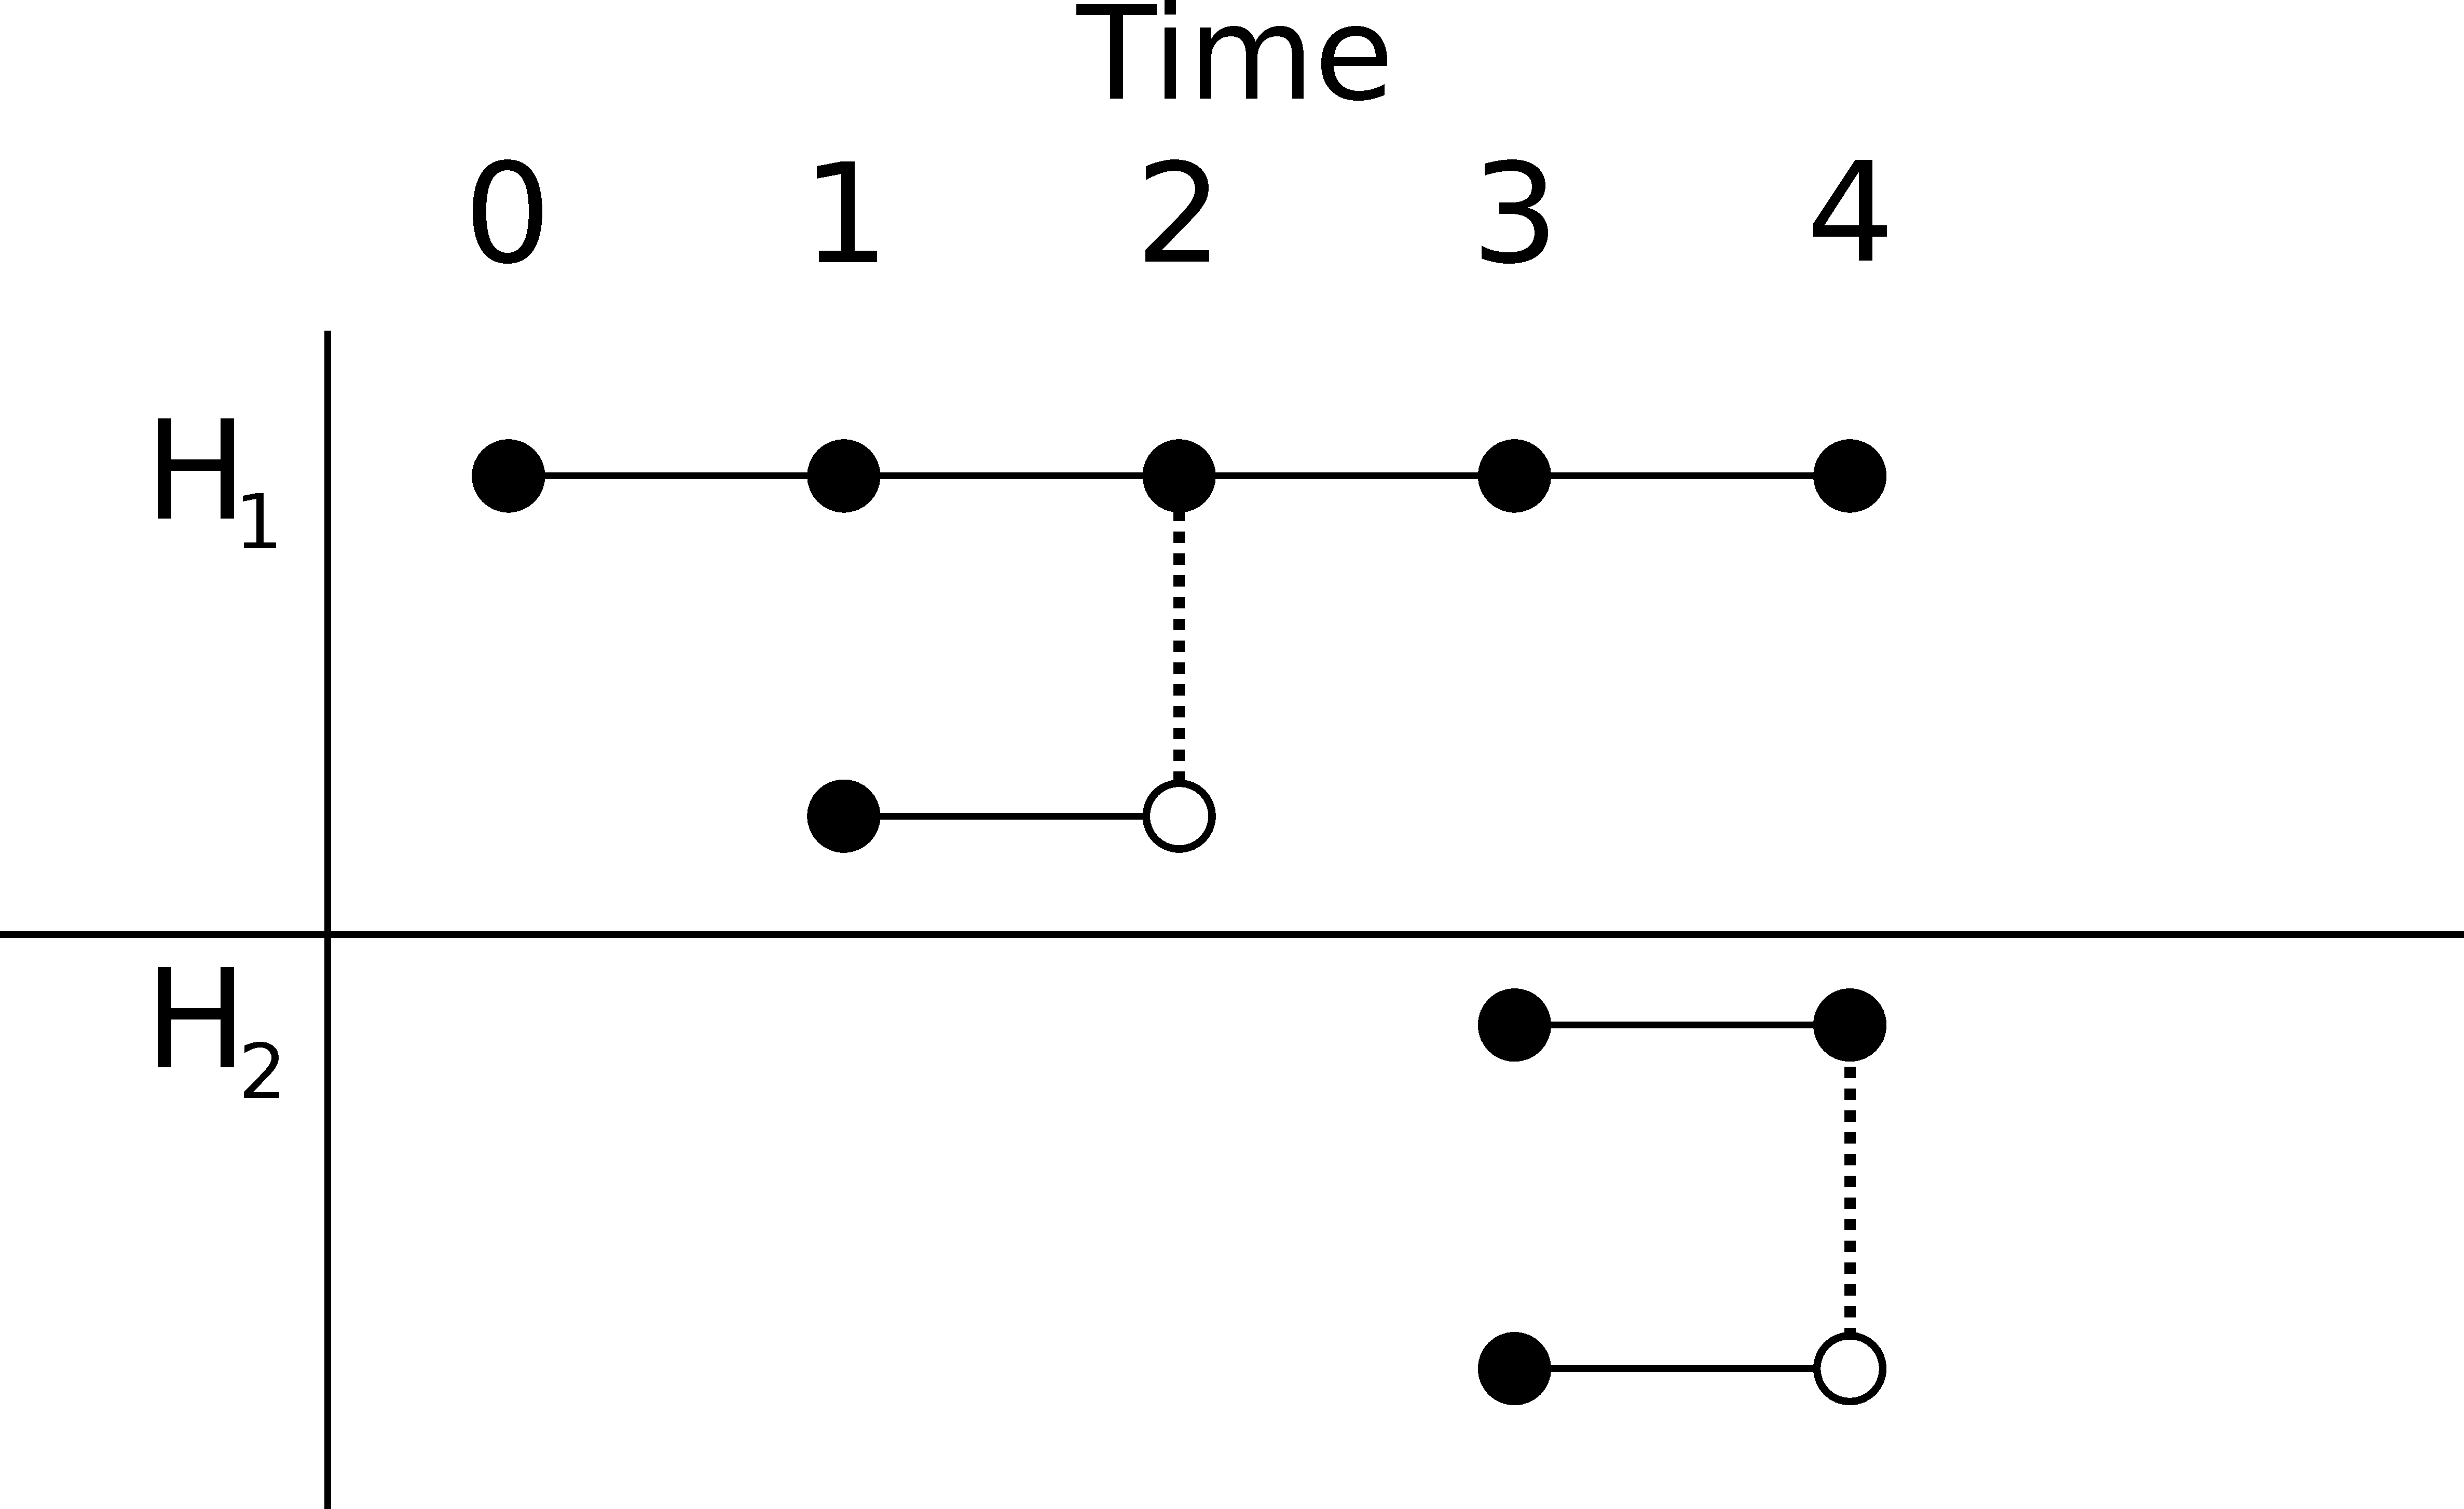
\includegraphics[scale=0.07]{./images/filtration/small/barcode.pdf}}}%
    \caption{Examples of visualising persistent homology of the filtration on Figure \ref{fig:example-filtration}.}%
    \label{fig:ph-viz}%
\end{figure}

% You can see in the digram that one 0th homology class is born at time $1$ and another one at time $2$. In time $3$ the class born at time $1$ merges with the class that is born at time $1$ because it is the younger class. In time $4$ on the other hand two cycles or 1st homology classes are born. One of them dies at time $5$ and the other one pesists. These events corresponds to the persistent homology pairs $(2, 3), (4, 5), (1, \infty)$ and $(4, \infty)$.

Now let us apply the general theory of persistent homology to a more familiar domain. Let $M$ be a simplicial mesh that is the triangulation of a bounded area in $\mathbb{R}^2$ and let $f: M \to \mathbb{R}$ be a linear interpolat based on the vertices of $M$. We would like to obtain a filtration of $M$ that we can analyse with persistent homology. The filtration that is proposed in the literature \cite{comp-topo} for manifolds and Morse functions is defined via the sublevel or superlevel sets of the manifold.

From Chapter 3 we know that $M$ is a manifold and that $f$ is a Morse function. The following claims hold:

\begin{itemize}
    \item $f$ has finitely many critical points,
    \item changes in the topology of the sublevel sets of $M$ happen only at critical points and
    \item critical points are at the vertices of $M$.
\end{itemize}

Therefore we need only consider the sublevel sets at the critical values of $f$. Let $c_1 < c_2 < ... < c_n$ be all critical values and let $M_{c_i} = f^{-1}((-\infty, c_i])$ be the sublevel sets at the critical values where we do not include all simplices which are not entirely contained in $M_{c_i}$ in order to obtain a simplicial complex. This lets us obtain a filtration of the sublevel sets:

$$ M_{c_1} \subseteq M_{c_2} \subseteq ... \subseteq M_{c_{n-1}} \subseteq M_{c_n} = M.$$

From this filtration we can produce the following sequence of homology groups and maps between them:

$$ H_n(M_{c_1}) \overset{i_*}{\longrightarrow} H_n(M_{c_2}) \overset{i_*}{\longrightarrow} ... \overset{i_*}{\longrightarrow} H_n(M_{c_{n-1}}) \overset{i_*}{\longrightarrow} H_n(M_{c_n}) = H_n(M).$$

If we had taken the superlevel sets of $M$ we would have obtained a different filtration. We will call that the descending filtration of $M$.

$$ H_n(M^{c_1}) \overset{i_*}{\longrightarrow} H_n(M^{c _2}) \overset{i_*}{\longrightarrow} ... \overset{i_*}{\longrightarrow} H_n(M^{c_{n-1}}) \overset{i_*}{\longrightarrow} H_n(M^{c_n}) = H_n(M).$$

We can use both filtration to compute the persistent homology of the ascending and descending filtrations of $M$.

% We are now able to compute both the contour tree and its branch decomposition and persistent homology. Our motivation behind doing so has been sparked by a quote from the original paper that introduced branch decomposition of contour trees \cite{ct-branch-decomp}. Branch decomposition results in a set of branches or equivalently pairings of critiral points of the contour tree. In the branch decomposition paper the importance of branches is based on their persistence as defined in the original paper that introduced persistent homology \cite{persistence-original}.

% This idea of the similarity between the two however has not been explained in detal nor explored further in the paper or in subsequent publications. We would like to explore it further. We would like to test whether the pairings produced from branch decomposition are the same as the pairings produced by persistent homology. We will do so by computing both on the same data sets and comparing the results to see how and why they differ. Before doing so however we must address an inconsistency between the two.
%
% The branch decomposition of the contour tree pair all critical points. Some critical points in persistent homology however are not "properly" paired. These are the ones that corespond to essential homology classes which have infinite persistence. To address this issue we will introduce an extension to persistent homology that "properly" pairs essential homology classes by assinging them with finite persistence.


\section{Extended Persistence}



% We have seen from the definition and computations of persistent homology that not all critical points of $M$ wil be paired.
%
% Furthermore the persistence of points that give birth to essential classes is not well defined because it is equal to $\infty$.
%
% Our goal in extending persistence it to devise a way to pair the essential homology classes with the remaining unpaired critical points \cite{persistence-extended}.

% will not be paired because they are never destroyed pass the final simplex in the filtration.
%
% This leads to incompleteness in the persistence pairings because persistence for some pa

% which we would to remedy. Our goal in extending persistence it to devise a way to pair the essential homology classes with the remaining unpaired critical points \cite{persistence-extended}.

% Let $M$ be a traingulation of a bounded area in $\mathbb{R}^2$ and let $f: M \to \mathbb{R}$ be a linear interpolat.

When $M$ is a triangulation of a bounded area in $\mathbb{R}^2$ and $f: M \to \mathbb{R}$ is a linear interpolat not all critical points are paired by persistent homology. Some are left out because pairs that include essential homology classes have infinite persistence. Such pairs only pair one critical point, not two. The purpose of extending persistence is to devise a way to pair the critical points that correspond to essential homology classes with remaining unpaired critical points \cite{persistence-extended}.

The main idea behind extended persistence is to follow the ascending filtration of persistent homology with a descending filtration. In the descending filtration we remember which the essential homology classes are. While in the descending filtration once we reach a class that is homologous to an essential class we consider it to be destroyed and thus paired. Extended persistence consists of two consecutive sequences. The first sequence is the made up of homology groups going up

$$ 0 \rightarrow H_n(M_{c_1}) \rightarrow H_n(M_{c_2}) \rightarrow ... \rightarrow H_n(M_{c_{n-1}}) \rightarrow H_n(M_{c_n}) =  H_n(M) .$$

Just like in ordinary persistence the linear maps between consecutive homology groups are induced by the inclusion maps between $M_{c_i} \subseteq M_{c_{i+1}}$. The second sequence is made up of relative homology groups that come back down:

$$ H_n(M) = H_n(M, M^{c_n}) \rightarrow H_n(M, M^{c_{n-1}}) \rightarrow... \rightarrow H_n(M, M^{c_{2}}) \rightarrow H_n(M, M^{c_{1}}) \rightarrow 0.$$

The linear maps between the relative homology groups in the relative sequence are induced by inclusion of pairs. The pairs $(M, M^{c_i})$ and $(M, M^{c_{i-1}})$ are such that $M^{c_i} \subseteq M^{c_{i-1}}$ and by Definition \ref{def:pairs} induce linear maps between $H_n(M, M^{c_i})$ and $H_n(M, M^{c_{i-1}})$. When we combine the two sequences at $H_n(M_{c_n}) =  H_n(M) = H_n(M, M^{c_n})$ we obtain the following single sequence:

$$ 0 \rightarrow H_n(M_{c_1}) \rightarrow ... \rightarrow H_n(M_{c_n}) = H_n(M, M^{c_n}) \rightarrow ... \rightarrow H_n(M, M^{c_{1}}) \rightarrow 0.$$

The extended persistence sequence of homology groups start from the trivial group and ends at the trivial group. This means that all classes that are born will eventually die in a finite amount of time steps. Extended persistent is symmetric. If we instead start with a descending filtration

$$ 0 \rightarrow H_n(M^{c_n}) \rightarrow H_n(M^{c_{n-1}}) \rightarrow ... \rightarrow H_n(M^{c_{2}}) \rightarrow H_n(M^{c_1}) =  H_n(M) $$
and follow that with a relative ascending filtration
$$ H_n(M) = H_n(M, M_{c_1}) \rightarrow H_n(M, M_{c_{2}}) \rightarrow... \rightarrow H_n(M, M_{c_{n-1}}) \rightarrow H_n(M, M_{c_{n}}) \rightarrow 0 $$
we would get the extended persistence of the descending filtration of $M$
$$ 0 \rightarrow H_n(M^{c_n}) \rightarrow ... \rightarrow H_n(M^{c_1}) = H_n(M, M_{c_1}) \rightarrow ... \rightarrow H_n(M, M_{c_n}) \rightarrow 0.$$

A good aid in understanding extended persistence is the Excision Theorem. We can use it compute the relative homology groups $H_n(M, M^{c_k})$ by computing the reduced homology groups of the quotient space $\overset{\sim}{H}_n(M / M^{c_k})$. We refer the reader \cite{folded-molecules} for more details examples of this.

% To see why this is true first observe that $i$ induces an identity map between $C(X)$ and $C(X)$. This idetity map takes $C_n(A)$ to $C_n(B)$ and so we can create a well defined map $i_\#: C(X, A) \to C(X, B)$ such that $i_\#([\sigma]_A) = [\sigma]_B$. This map clearly commuted with the relative boundary map, therefore it induces a linear map on the relative homology groups.

% is an identity map then $i_\#(A) \subseteq$

% To see why this is true observe that the identity map $i: X \to X$ induces a linear map $i_\#: C(X, A) \to C(X, B)$ because the

% This implies that



% The homomorphism is induced by taking the simplicies of a chain through the simplicial map and the considering the homology class the chain ends up in (if any). Detail on this can be found in \cite{combinatorial-algebraic-topology}. We will further expand this definition to also cover relative chain maps and relative homologies.
%
% \begin{defn} Let $X$ and $Y$ be two simplical complexes and let $A \subseteq X$ and $B \subseteq Y$ be two subcomplexes. Let $f: X \to Y$ be a simplicial map such that $f(A) \subseteq B$. Then $f$ induces a homomorphism $f_*: H_n(X, A) \to H_n(Y, B)$ for all $n \in \{0, 1, 2, ...\}$. \end{defn}
%
%
%
% We will further expand this definition to also cover relative chain maps and relative homologies.
%
% \begin{defn} Let $X$ and $Y$ be two simplical complexes and let $A \subseteq X$ and $B \subseteq Y$ be two subcomplexes. Let $f: X \to Y$ be a simplicial map such that $f(A) \subseteq B$. Then $f$ induces a homomorphism $f_*: H_n(X, A) \to H_n(Y, B)$ for all $n \in \{0, 1, 2, ...\}$. \end{defn}
%
% We will use the shorthand $f: (X, A) \to (Y, B)$ for functions that satisfy the criteria of this definition. The function $f$ is called a simplicial map between simplicial pairs (analogous to continuous map between topological pairs in \cite{algebraic-topology}).


% We will devote this final section to introducing simplicial maps between chain complexes and how they induce linear maps between the homology and relative homology groups of the chain complexes. We will begin by defining simplicial maps \cite{combinatorial-algebraic-topology}.
%
% \begin{defn} Let $X$ and $Y$ be two simplicial complexes. A function $f: X \to Y$ is a simplical map if it takes every simplex $\sigma$ of $X$ to a simplex $f(\sigma)$ of $Y$ and furthermore the dimensions of $\sigma$ and $f(\sigma)$ are equal.
% \end{defn}
%
% The definition we use here is more restrictive than that in \cite{combinatorial-algebraic-topology} because it requires that simplicial maps preserve the dimensions of simplicies. We have altered the definition for two reasons. First to simplify the treatment of the subject and second because we will only be making use of inclusion maps between a subcomplex and a complex.
%
% Simplicial maps play an important role in Homology. If we establish a simplicial map between two simplicial complexes we can use it to obtain a map between the chain groups of the simplical complexes. We will such a map a chain map.
%
% \begin{defn} Let $X$ and $Y$ be two simplical complexes and $f: X \to Y$ be a simplicial map. Then $f$ induces a chain map $f_\#: C_n(X) \to C_n(Y)$ for all $n \in \mathbb{Z}$. \end{defn}
%
% The chain map is induced by linearly extending $f$ to chains in the chain groups and applying it to simplicies of $X$. It is defined as $f_\#(\sum_ia_i\sigma_i) = \sum_i a_i f(\sigma_i)$. Upon obtaining chain maps between the chain complexes of $X$ and $Y$ we can a step further a induce a linear map between the homology groups of $X$ and $Y$.
%
% \begin{defn} Let $X$ and $Y$ be two simplical complexes and $f: X \to Y$ be a simplicial map. Then $f$ induces a linear map $f_*: H_n(X) \to H_n(Y)$ such that $f_*([\sigma]) = [f_\#(\sigma)]$ for all $n \in \mathbb{Z}$. \end{defn}
%
% Where $[\sigma]$ is the homology group is a an n-chain in $C_n(X)$ and $[f_\#(\sigma)]$ is an

% We define such that $f_#(\sigma) = f(\sigma)$


% where $\sigma$ is a simplex of $X$ and $f(\sigma)$ is a simplex of $Y$ because $f$ is a simplicial map.

% Simplicial maps play an important role in Homology. If we establish a simplicial map between two simplicial complexes we can use it to obtain a map between the homology groups of the simplicial maps. This new map is called an incuded linear map.

% \begin{defn} Let $X$ and $Y$ be two simplical complexes and $f: X \to Y$ be a simplicial map. Then $f$ induces a linear map $f_*: H_n(X) \to H_n(Y)$ such that $f_*([\sigma]) = [f(\sigma)]$ for all $n \in \mathbb{Z}$. \end{defn}

% In the definition $[\sigma]$ is the homology class of $\sigma$ in $H_n(X)$ and $[f(\sigma)]$ is the homology class of $f(\sigma)$ in $H_n(Y)$.



% The two most important observations we can make based on this defitions are the following:
%
% \begin{itemize}
%     \item The composition of two simplicial maps is simplicial.
%     \item When $Y$ is a subcompex of $X$ the inclusion map is a simplicial map.
% \end{itemize}
%
%

% The reason why we introduced simplicial maps is so that we can pose the following question. If there is a simplical map between two simplicial complexes, can we use it to relate their homology classes? The answer is yes, we can thanks to \cite{combinatorial-algebraic-topology}!
%
%

%
% \begin{defn} Let $X$ and $Y$ be two simplical complexes and $f: X \to Y$ be a simplicial map. Then $f$ induces a homomorphism $f_*: H_n(X) \to H_n(Y)$ for all $n \in \{0, 1, 2, ...\}$. \end{defn}
%
% The homomorphism is induced by taking the simplicies of a chain through the simplicial map and the considering the homology class the chain ends up in (if any). Detail on this can be found in \cite{combinatorial-algebraic-topology}. We will further expand this definition to also cover relative chain maps and relative homologies.
%
% \begin{defn} Let $X$ and $Y$ be two simplical complexes and let $A \subseteq X$ and $B \subseteq Y$ be two subcomplexes. Let $f: X \to Y$ be a simplicial map such that $f(A) \subseteq B$. Then $f$ induces a homomorphism $f_*: H_n(X, A) \to H_n(Y, B)$ for all $n \in \{0, 1, 2, ...\}$. \end{defn}
%
% We will use the shorthand $f: (X, A) \to (Y, B)$ for functions that satisfy the criteria of this definition. The function $f$ is called a simplicial map between simplicial pairs (analogous to continuous map between topological pairs in \cite{algebraic-topology}).


% The homomorphism is induced by running the relative homology classes through the simplicial map and recording which class their image lands in. The primary type of map we will use in this chapter is a specific kind of simplicial map - the inclusion map. The reason for this will become clear in the following section. In the case of absolute homology when $X$ is a simplicial complex and $A$ is a subcomplex of $X$ there is a natural inclusion map $i: A \to X$ which is injective but not necessarily surjective. It takes the simplicies of $A$ to exactly the same simplicies of $X$ and leaves the simplicies outside of $A$ untouched.
%
% We shall define the inclusion of relative homology analogously. Let $B$ be another subcomplex of $X$ such that $A$ is also a subcomplex of $B$, or $A \subseteq B \subseteq X$. Then let $i : X \to X$ be the identity map. As $A \subseteq B$ then the restriction $i_A: A \to B$ is a well defined function and therefore $i(A) \subseteq B$. Therefore there is a map $i$ between the pairs $(X, A)$ and $(X, B)$ such that $i(A) \subseteq B$ by the previous definition this map induces a homomorphism $i_* : H_n(X, A) \to H_n(X, B)$.


% Before introducing ourselves with persistent homology we will take a slight detour in order to introduce the last piece that we are missing to enable its construction. There is a general result in singular homology that shows the interaction of continuous maps and homomorphisms between homology groups.
%
% \begin{defn} Let $X$ and $Y$ be two topological spaces. Let $f: X \to Y$ be a continuous function. Then $f$ induces a homomorphism $f_*: H_n(X) \to H_n(Y)$ for all $n \in \{0, 1, 2, ...\}$. \end{defn}
%
% This means that if we have a continuous function between two spaces we can immediately associate the homology classes of $X$ to those of $Y$. All we have to do to obtain the induced map is to compose the simplices with the continuous function $f$. The details of this process are outlines in \cite{algebraic-topology}.
%
%
% This general result is not appropriate for simplicial complexes. WHY?! We need a more tracktable definition to aid us in our computation. We will thus present the following combinatorially flavoured definition given by \cite{combinatorial-algebraic-topology}.
